
%% bare_jrnl.tex
%% V1.3
%% 2007/01/11
%% by Michael Shell
%% see http://www.michaelshell.org/
%% for current contact information.
%%
%% This is a skeleton file demonstrating the use of IEEEtran.cls
%% (requires IEEEtran.cls version 1.7 or later) with an IEEE journal paper.
%%
%% Support sites:
%% http://www.michaelshell.org/tex/ieeetran/
%% http://www.ctan.org/tex-archive/macros/latex/contrib/IEEEtran/
%% and
%% http://www.ieee.org/



% *** Authors should verify (and, if needed, correct) their LaTeX system  ***
% *** with the testflow diagnostic prior to trusting their LaTeX platform ***
% *** with production work. IEEE's font choices can trigger bugs that do  ***
% *** not appear when using other class files.                            ***
% The testflow support page is at:
% http://www.michaelshell.org/tex/testflow/


%%*************************************************************************
%% Legal Notice:
%% This code is offered as-is without any warranty either expressed or
%% implied; without even the implied warranty of MERCHANTABILITY or
%% FITNESS FOR A PARTICULAR PURPOSE! 
%% User assumes all risk.
%% In no event shall IEEE or any contributor to this code be liable for
%% any damages or losses, including, but not limited to, incidental,
%% consequential, or any other damages, resulting from the use or misuse
%% of any information contained here.
%%
%% All comments are the opinions of their respective authors and are not
%% necessarily endorsed by the IEEE.
%%
%% This work is distributed under the LaTeX Project Public License (LPPL)
%% ( http://www.latex-project.org/ ) version 1.3, and may be freely used,
%% distributed and modified. A copy of the LPPL, version 1.3, is included
%% in the base LaTeX documentation of all distributions of LaTeX released
%% 2003/12/01 or later.
%% Retain all contribution notices and credits.
%% ** Modified files should be clearly indicated as such, including  **
%% ** renaming them and changing author support contact information. **
%%
%% File list of work: IEEEtran.cls, IEEEtran_HOWTO.pdf, bare_adv.tex,
%%                    bare_conf.tex, bare_jrnl.tex, bare_jrnl_compsoc.tex
%%*************************************************************************

% Note that the a4paper option is mainly intended so that authors in
% countries using A4 can easily print to A4 and see how their papers will
% look in print - the typesetting of the document will not typically be
% affected with changes in paper size (but the bottom and side margins will).
% Use the testflow package mentioned above to verify correct handling of
% both paper sizes by the user's LaTeX system.
%
% Also note that the "draftcls" or "draftclsnofoot", not "draft", option
% should be used if it is desired that the figures are to be displayed in
% draft mode.
%
\documentclass[conference]{IEEEtran}
%
% If IEEEtran.cls has not been installed into the LaTeX system files,
% manually specify the path to it like:
% \documentclass[journal]{../sty/IEEEtran}

% Some very useful LaTeX packages include:
% (uncomment the ones you want to load)


% *** MISC UTILITY PACKAGES ***
%
%\usepackage{ifpdf}
% Heiko Oberdiek's ifpdf.sty is very useful if you need conditional
% compilation based on whether the output is pdf or dvi.
% usage:
% \ifpdf
%   % pdf code
% \else
%   % dvi code
% \fi
% The latest version of ifpdf.sty can be obtained from:
% http://www.ctan.org/tex-archive/macros/latex/contrib/oberdiek/
% Also, note that IEEEtran.cls V1.7 and later provides a builtin
% \ifCLASSINFOpdf conditional that works the same way.
% When switching from latex to pdflatex and vice-versa, the compiler may
% have to be run twice to clear warning/error messages.

% *** CITATION PACKAGES ***
%
%\usepackage{cite}
% cite.sty was written by Donald Arseneau
% V1.6 and later of IEEEtran pre-defines the format of the cite.sty package
% \cite{} output to follow that of IEEE. Loading the cite package will
% result in citation numbers being automatically sorted and properly
% "compressed/ranged". e.g., [1], [9], [2], [7], [5], [6] without using
% cite.sty will become [1], [2], [5]--[7], [9] using cite.sty. cite.sty's
% \cite will automatically add leading space, if needed. Use cite.sty's
% noadjust option (cite.sty V3.8 and later) if you want to turn this off.
% cite.sty is already installed on most LaTeX systems. Be sure and use
% version 4.0 (2003-05-27) and later if using hyperref.sty. cite.sty does
% not currently provide for hyperlinked citations.
% The latest version can be obtained at:
% http://www.ctan.org/tex-archive/macros/latex/contrib/cite/
% The documentation is contained in the cite.sty file itself.

% *** GRAPHICS RELATED PACKAGES ***
%
\ifCLASSINFOpdf
  \usepackage[pdftex]{graphicx}
  % declare the path(s) where your graphic files are
  \graphicspath{{../figures/}}
  % and their extensions so you won't have to specify these with
  % every instance of \includegraphics
  % \DeclareGraphicsExtensions{.pdf,.jpeg,.png}
\else
  % or other class option (dvipsone, dvipdf, if not using dvips). graphicx
  % will default to the driver specified in the system graphics.cfg if no
  % driver is specified.
  \usepackage[dvips]{graphicx}
  % declare the path(s) where your graphic files are
  % \graphicspath{{../eps/}}
  % and their extensions so you won't have to specify these with
  % every instance of \includegraphics
  % \DeclareGraphicsExtensions{.eps}
\fi
\usepackage{xcolor}

% *** MATH PACKAGES ***
%
\usepackage[cmex10]{amsmath}
\usepackage{amsfonts}
% A popular package from the American Mathematical Society that provides
% many useful and powerful commands for dealing with mathematics. If using
% it, be sure to load this package with the cmex10 option to ensure that
% only type 1 fonts will utilized at all point sizes. Without this option,
% it is possible that some math symbols, particularly those within
% footnotes, will be rendered in bitmap form which will result in a
% document that can not be IEEE Xplore compliant!
%
% Also, note that the amsmath package sets \interdisplaylinepenalty to 10000
% thus preventing page breaks from occurring within multiline equations. Use:
\interdisplaylinepenalty=2500
% after loading amsmath to restore such page breaks as IEEEtran.cls normally
% does. amsmath.sty is already installed on most LaTeX systems. The latest
% version and documentation can be obtained at:
% http://www.ctan.org/tex-archive/macros/latex/required/amslatex/math/

% *** SPECIALIZED LIST PACKAGES ***
%
%\usepackage{algorithmic}
% algorithmic.sty was written by Peter Williams and Rogerio Brito.
% This package provides an algorithmic environment fo describing algorithms.
% You can use the algorithmic environment in-text or within a figure
% environment to provide for a floating algorithm. Do NOT use the algorithm
% floating environment provided by algorithm.sty (by the same authors) or
% algorithm2e.sty (by Christophe Fiorio) as IEEE does not use dedicated
% algorithm float types and packages that provide these will not provide
% correct IEEE style captions. The latest version and documentation of
% algorithmic.sty can be obtained at:
% http://www.ctan.org/tex-archive/macros/latex/contrib/algorithms/
% There is also a support site at:
% http://algorithms.berlios.de/index.html
% Also of interest may be the (relatively newer and more customizable)
% algorithmicx.sty package by Szasz Janos:
% http://www.ctan.org/tex-archive/macros/latex/contrib/algorithmicx/

\usepackage{enumerate}

% *** ALIGNMENT PACKAGES ***
%
\usepackage{array}
% Frank Mittelbach's and David Carlisle's array.sty patches and improves
% the standard LaTeX2e array and tabular environments to provide better
% appearance and additional user controls. As the default LaTeX2e table
% generation code is lacking to the point of almost being broken with
% respect to the quality of the end results, all users are strongly
% advised to use an enhanced (at the very least that provided by array.sty)
% set of table tools. array.sty is already installed on most systems. The
% latest version and documentation can be obtained at:
% http://www.ctan.org/tex-archive/macros/latex/required/tools/

\usepackage{mdwmath}
\usepackage{mdwtab}
% Also highly recommended is Mark Wooding's extremely powerful MDW tools,
% especially mdwmath.sty and mdwtab.sty which are used to format equations
% and tables, respectively. The MDWtools set is already installed on most
% LaTeX systems. The lastest version and documentation is available at:
% http://www.ctan.org/tex-archive/macros/latex/contrib/mdwtools/

% IEEEtran contains the IEEEeqnarray family of commands that can be used to
% generate multiline equations as well as matrices, tables, etc., of high
% quality.

\usepackage{eqparbox}
% Also of notable interest is Scott Pakin's eqparbox package for creating
% (automatically sized) equal width boxes - aka "natural width parboxes".
% Available at:
% http://www.ctan.org/tex-archive/macros/latex/contrib/eqparbox/

% *** SUBFIGURE PACKAGES ***
\usepackage[tight,footnotesize]{subfigure}
% subfigure.sty was written by Steven Douglas Cochran. This package makes it
% easy to put subfigures in your figures. e.g., "Figure 1a and 1b". For IEEE
% work, it is a good idea to load it with the tight package option to reduce
% the amount of white space around the subfigures. subfigure.sty is already
% installed on most LaTeX systems. The latest version and documentation can
% be obtained at:
% http://www.ctan.org/tex-archive/obsolete/macros/latex/contrib/subfigure/
% subfigure.sty has been superceeded by subfig.sty.

\usepackage[font=footnotesize, caption=false]{subfig}
% subfig.sty, also written by Steven Douglas Cochran, is the modern
% replacement for subfigure.sty. However, subfig.sty requires and
% automatically loads Axel Sommerfeldt's caption.sty which will override
% IEEEtran.cls handling of captions and this will result in nonIEEE style
% figure/table captions. To prevent this problem, be sure and preload
% caption.sty with its "caption=false" package option. This is will preserve
% IEEEtran.cls handing of captions. Version 1.3 (2005/06/28) and later 
% (recommended due to many improvements over 1.2) of subfig.sty supports
% the caption=false option directly:
%\usepackage[caption=false,font=footnotesize]{subfig}
%
% The latest version and documentation can be obtained at:
% http://www.ctan.org/tex-archive/macros/latex/contrib/subfig/
% The latest version and documentation of caption.sty can be obtained at:
% http://www.ctan.org/tex-archive/macros/latex/contrib/caption/




% *** FLOAT PACKAGES ***
%
%\usepackage{fixltx2e}
% fixltx2e, the successor to the earlier fix2col.sty, was written by
% Frank Mittelbach and David Carlisle. This package corrects a few problems
% in the LaTeX2e kernel, the most notable of which is that in current
% LaTeX2e releases, the ordering of single and double column floats is not
% guaranteed to be preserved. Thus, an unpatched LaTeX2e can allow a
% single column figure to be placed prior to an earlier double column
% figure. The latest version and documentation can be found at:
% http://www.ctan.org/tex-archive/macros/latex/base/

%\usepackage{stfloats}
% stfloats.sty was written by Sigitas Tolusis. This package gives LaTeX2e
% the ability to do double column floats at the bottom of the page as well
% as the top. (e.g., "\begin{figure*}[!b]" is not normally possible in
% LaTeX2e). It also provides a command:
%\fnbelowfloat
% to enable the placement of footnotes below bottom floats (the standard
% LaTeX2e kernel puts them above bottom floats). This is an invasive package
% which rewrites many portions of the LaTeX2e float routines. It may not work
% with other packages that modify the LaTeX2e float routines. The latest
% version and documentation can be obtained at:
% http://www.ctan.org/tex-archive/macros/latex/contrib/sttools/
% Documentation is contained in the stfloats.sty comments as well as in the
% presfull.pdf file. Do not use the stfloats baselinefloat ability as IEEE
% does not allow \baselineskip to stretch. Authors submitting work to the
% IEEE should note that IEEE rarely uses double column equations and
% that authors should try to avoid such use. Do not be tempted to use the
% cuted.sty or midfloat.sty packages (also by Sigitas Tolusis) as IEEE does
% not format its papers in such ways.


%\ifCLASSOPTIONcaptionsoff
%  \usepackage[nomarkers]{endfloat}
% \let\MYoriglatexcaption\caption
% \renewcommand{\caption}[2][\relax]{\MYoriglatexcaption[#2]{#2}}
%\fi
% endfloat.sty was written by James Darrell McCauley and Jeff Goldberg.
% This package may be useful when used in conjunction with IEEEtran.cls'
% captionsoff option. Some IEEE journals/societies require that submissions
% have lists of figures/tables at the end of the paper and that
% figures/tables without any captions are placed on a page by themselves at
% the end of the document. If needed, the draftcls IEEEtran class option or
% \CLASSINPUTbaselinestretch interface can be used to increase the line
% spacing as well. Be sure and use the nomarkers option of endfloat to
% prevent endfloat from "marking" where the figures would have been placed
% in the text. The two hack lines of code above are a slight modification of
% that suggested by in the endfloat docs (section 8.3.1) to ensure that
% the full captions always appear in the list of figures/tables - even if
% the user used the short optional argument of \caption[]{}.
% IEEE papers do not typically make use of \caption[]'s optional argument,
% so this should not be an issue. A similar trick can be used to disable
% captions of packages such as subfig.sty that lack options to turn off
% the subcaptions:
% For subfig.sty:
% \let\MYorigsubfloat\subfloat
% \renewcommand{\subfloat}[2][\relax]{\MYorigsubfloat[]{#2}}
% For subfigure.sty:
% \let\MYorigsubfigure\subfigure
% \renewcommand{\subfigure}[2][\relax]{\MYorigsubfigure[]{#2}}
% However, the above trick will not work if both optional arguments of
% the \subfloat/subfig command are used. Furthermore, there needs to be a
% description of each subfigure *somewhere* and endfloat does not add
% subfigure captions to its list of figures. Thus, the best approach is to
% avoid the use of subfigure captions (many IEEE journals avoid them anyway)
% and instead reference/explain all the subfigures within the main caption.
% The latest version of endfloat.sty and its documentation can obtained at:
% http://www.ctan.org/tex-archive/macros/latex/contrib/endfloat/
%
% The IEEEtran \ifCLASSOPTIONcaptionsoff conditional can also be used
% later in the document, say, to conditionally put the References on a 
% page by themselves.


% *** PDF, URL AND HYPERLINK PACKAGES ***
%
\usepackage{url}
% url.sty was written by Donald Arseneau. It provides better support for
% handling and breaking URLs. url.sty is already installed on most LaTeX
% systems. The latest version can be obtained at:
% http://www.ctan.org/tex-archive/macros/latex/contrib/misc/
% Read the url.sty source comments for usage information. Basically,
% \url{my_url_here}.


% *** Do not adjust lengths that control margins, column widths, etc. ***
% *** Do not use packages that alter fonts (such as pslatex).         ***
% There should be no need to do such things with IEEEtran.cls V1.6 and later.
% (Unless specifically asked to do so by the journal or conference you plan
% to submit to, of course. )


% correct bad hyphenation here
%\hyphenation{op-tical net-works semi-conduc-tor}

%%%%%%%%%%%%%%%%%%%%%%%%%%%%%%%%%%%%%%%%%%%%%%%%%
%%%%%%%SPECIFIC TO MParticle.tex (user-defined commands) %%%%%%%%%%%%%%%
%%%%%%%%%%%%%%%%%%%%%%%%%%%%%%%%%%%%%%%%%%%%%%%%%


\newcommand{\expectation}[1]{\mathbb{E}\Big\{ #1 \Big\}}	
\global\long\def\link{l}
\global\long\def\numlinks{N}
\global\long\def\linkset{\mathcal{L}}
\global\long\def\internallinks{\linkset_{\text{int}}}
\global\long\def\entrylinks{\linkset_{\text{ent}}}
\global\long\def\exitlinks{\linkset_{\text{ex}}}

\newenvironment{Def}[1][Definition]{\begin{trivlist}
\item[\hskip \labelsep {\bfseries #1}]}{\end{trivlist}}

\newtheorem{Thm}{\textbf{Theorem}}
\newtheorem{Prop}[Thm]{\textbf{Property}}
\newtheorem{Lem}[Thm]{\textbf{Lemma}}



\renewcommand{\IEEElabelindentfactori}{.5}
%\renewcommand{\iedlistdecl}{\settowidth{\labelsep}{H}}
\setlength{\IEEEilabelindent}{0pt}
\setlength{\IEEEiednormlabelsep}{3pt}
\setlength{\itemsep}{.5pt}
%\setlabelwidth{0}
%%%%%%%%%%%%%%%%%%%%%%%%%%%%%%%%%%%%%%%%%%%%%%%%%
%%%%%%%%%%%%%%%%%%%%%%%%%%%%%%%%%%%%%%%%%%%%%%%%%
%%%%%%%%%%%%%%%%%%%%%%%%%%%%%%%%%%%%%%%%%%%%%%%%%

%%%%%%%%%%%%%%%%%%%%%%%%%%%%%%%%%%%%%%%%%%%%%%%%%
%Hack pour boxalert
%%%%%%%%%%%%%%%%%%%%%%%%%%%%%%%%%%%%%%%%%%%%%%%%%
%\usepackage[latin9]{inputenc}
%%%%%%%%%%%%%%%%%%%%%%%%%%%%%%%%%%%%%%%%%%%%%%%%%


\begin{document}

\title{Stability of Modified Max Pressure Controller with Application to Signalized Traffic Networks
\vspace{-.2em}}
% can use linebreaks \\ within to get better formatting as desired
\author{Thomas~Pumir,~%~\IEEEmembership{Student Member,~IEEE,}
        Leah~Anderson,~%~\IEEEmembership{Student Member,~IEEE,}
        Dimitrios~Triantafyllos,~
        and~Alexandre~M.~Bayen
        \vspace{-.5em}%,~\IEEEmembership{Member,~IEEE}% <-this % stops a space
%\thanks{T.~Pumir and A.~Bayen are with the Dept.
%of Electrical Engineering and Computer Science and L.~Anderson is with the Dept. of Civil and Environmental Engineering at the University of California, Berkeley, CA; Corresponding e-mail: thomas.pumir@berkeley.edu}% <-this % stops a space
%\thanks{This work was sponsored by the California Department of Transportation under the Connected Corridors program at PATH, UC Berkeley.  }% <-this % stops a space
}

% note the % following the last \IEEEmembership and also \thanks - 
% these prevent an unwanted space from occurring between the last author name
% and the end of the author line. i.e., if you had this:
% 
% \author{....lastname \thanks{...} \thanks{...} }
%                     ^------------^------------^----Do not want these spaces!
%
% a space would be appended to the last name and could cause every name on that
% line to be shifted left slightly. This is one of those "LaTeX things". For
% instance, "\textbf{A} \textbf{B}" will typeset as "A B" not "AB". To get
% "AB" then you have to do: "\textbf{A}\textbf{B}"
% \thanks is no different in this regard, so shield the last } of each \thanks
% that ends a line with a % and do not let a space in before the next \thanks.
% Spaces after \IEEEmembership other than the last one are OK (and needed) as
% you are supposed to have spaces between the names. For what it is worth,
% this is a minor point as most people would not even notice if the said evil
% space somehow managed to creep in.



% The paper headers
\markboth{Journal NAME,~Vol.~NUM, No.~NUM, MONTH~2014}%
{OTHER PAPER HEADER (SHORTENED TITLE, JOURNAL NAME, ETC)}
% The only time the second header will appear is for the odd numbered pages
% after the title page when using the twoside option.
% 
% *** Note that you probably will NOT want to include the author's ***
% *** name in the headers of peer review papers.                   ***
% You can use \ifCLASSOPTIONpeerreview for conditional compilation here if
% you desire.


% If you want to put a publisher's ID mark on the page you can do it like
% this:
%\IEEEpubid{0000--0000/00\$00.00~\copyright~2007 IEEE}
% Remember, if you use this you must call \IEEEpubidadjcol in the second
% column for its text to clear the IEEEpubid mark.

% use for special paper notices
%\IEEEspecialpapernotice{(Invited Paper)}

\maketitle
\setlength{\belowdisplayskip}{4pt} \setlength{\belowdisplayshortskip}{1pt}
\setlength{\abovedisplayskip}{4pt} \setlength{\abovedisplayshortskip}{1pt}
%\abovedisplayskip=6pt plus 3pt minus 4pt
%\abovedisplayshortskip=6pt plus 3pt
%\belowdisplayskip=6pt plus 3pt minus 4pt
%\belowdisplayshortskip=6pt plus 3pt minus 4pt
\begin{abstract}
% !TEX root = ./MParticle_resubmit.tex
This work describes a type of distributed feedback control algorithm that acts on a vertical queueing network where flow dynamics may greatly outpace the rate of feedback and actuation. The modeled network has a known, finite set of feasible actuations for the binary controllers located at each network node. It also has known expected demands, split ratios, and maximum service rates. Previous work proposed the application of a max pressure controller to maximize throughput on such a network without the need for centralized computation of a control policy. Here, we extend the max pressure controller to a practical scenario.
%where the frequency of actuation is limited relative to the more rapid timescale of queue formation and dissipation. 
%Specifically, we extend the feedback cycle so that control can only be modified at a rate much slower than that of the network's queue dynamics. We then extend the set of allowable controllers in this setting to any convex combination of available signal phases to account for signal changes within a single signal ``cycle''. We show that the proposed extended max pressure controllers stabilize the network (queue lengths remain bounded in expectation) given slight restrictions on admissible network demand flows.  
Specifically, we extend the controller so as to satisfy practical constraints on switching and minimum actuation guarantees. Fundamentally, we alter the formulation of max pressure to a setting where the controller may only update at a rate significantly slower than the dynamics of queue formation. However, the set of allowable controllers is extended to any convex combination of available signal phases to account for signal changes within a single signal ``cycle''. We show that this proposed extended max pressure controllers stabilize the network (queue lengths remain bounded in expectation) given slightly increased restrictions on admissible network demand flows.  
This work is motivated by the application of controlling traffic signals on arterial road networks. Max pressure provides an intriguing alternative to existing feedback control systems due to its theoretical guarantees, but cannot be directly applied as originally formulated due to hardware and safety constraints. We ultimately apply our extension of max pressure to a simulation of an existing arterial roadway and provide comparison to the control policy that is currently deployed on this site. 

%
%Designing efficient control of signalized intersections on road traffic networks is becoming an increasingly urgent issue in urban areas where vehicular traffic is nearing the capacity of available infrastructure.  Many currently deployed algorithms are not capable of reacting to changes in demand beyond gradual ``time of day'' variations, and thus cannot effectively handle the surges caused by nearby incidents or other common but unpredictable events. This work provides a distributed, reactive control algorithm that acts on a vertical queueing network controlled by binary signals at each internal node. The modeled network has known expected demands, split ratios and maximum service rates. Previous work proposed the application of a max pressure controller to maximize throughput on such a network without the need for centralized computation of a control policy. Here, we extend the max pressure controller to a more practical control scenario where actuator hardware and safety regulations limit the frequency of actuation relative to the more rapid timescale of queue formation and dissipation. Specifically, we extend the feedback cycle so that control can only be modified at a rate much slower than that of the network's queue dynamics. We then extend the set of allowable controllers in this setting to any convex combination of available signal phases to account for signal changes within a single signal ``cycle''. We show that the proposed extended max pressure controllers stabilize the network (queue lengths remain bounded in expectation) given slight restrictions on admissible network demand flows.  
%

\end{abstract}
% IEEEtran.cls defaults to using nonbold math in the Abstract.
% This preserves the distinction between vectors and scalars. However,
% if the journal you are submitting to favors bold math in the abstract,
% then you can use LaTeX's standard command \boldmath at the very start
% of the abstract to achieve this. Many IEEE journals frown on math
% in the abstract anyway.
% Note that keywords are not normally used for peerreview papers.
\begin{IEEEkeywords}
max pressure, vertical queueing network, network stability, adaptive signal control, arterial modeling
\end{IEEEkeywords}
% For peer review papers, you can put extra information on the cover
% page as needed:
% \ifCLASSOPTIONpeerreview
% \begin{center} \bfseries EDICS Category: 3-BBND \end{center}
% \fi
%
% For peerreview papers, this IEEEtran command inserts a page break and
% creates the second title. It will be ignored for other modes.
\IEEEpeerreviewmaketitle
% !TEX root = ./MParticle_resubmit.tex
\section{Introduction}

%The expansion of transportation networks over the past twenty years has motivated much study on the performance of queuing networks. 
This article investigates the design and stability of decentralized controller for vertical queueing networks. In a \emph{vertical queueing network}, agents traveling across the network are stored in ``point queues'' which do not inhabit a ``horizontal'' position along the length of a network edge, but instead are considered to be stored in ``vertical'' stacks at each node. Such models are inherited from fields such as supply chain management or internet routing, but are also representative of signalized urban traffic networks \cite{Aboudolas2009}\cite{vandenBerg2003}\cite{Zhang2013}.  The concept of a \emph{stabilizing} network controller, or one which ensures that the mean length of all queues in the network remain bounded, is relevant to many applications such as communications networks \cite{Giaccone2005}\cite{Neely2005}\cite{Pajic2013} or industrial systems \cite{Dai2005}\cite{Egerstedt2002}\cite{Brockett1995}\cite{Ishii2001}.

In the present work we examine a vertical queueing model in which only a finite set of non-conflicting turning movements (or \emph{phases}) can be permitted to flow simultaneously across each network node. Phase actuation is dictated by a controller such as a traffic light. Specifically, we consider application of a \emph{max pressure controller}. 

Max Pressure is a distributed network control policy derived from the concept of a ``back pressure controller'', which was first studied in the context of routing packets through a multi-hop communications network \cite{Tassiulas1992}. The idea was applied to road traffic management more recently by Varaiya \cite{Varaiya2013} as well as Wongpiromsarn et al. \cite{Wongpiromsarn2012}. The concept of max pressure control is intuitive: at each intersection, priority is given to the signal phase which will be able to service the most traffic given knowledge of both available upstream demand and the subsequent feasibility of downstream queues. It is a particularly attractive concept for control of a signalized urban traffic network because it can be operated in a distributed manner on local controller hardware but still provides theoretical guarantees on network-wide performance. Variaya's original formulation of this controller, however, does not fully consider the practical limitations on the rate of queue measurement and signal actuation in vehicle traffic networks. For example, a standard max pressure controller has no bound on the rate of signal switches which may occur relative to the rate of modeled queue formation and dissipation in the network. In implementation, a traffic signal incurs a penalty upon every change in actuation in the form of capacity loss due to ``intersection clearance time'': a 2-3 second period where all movements are given a red light in order to allow traffic from the previous phase to clear the intersection before possibly conflicting traffic can be permitted to enter. Max pressure also lacks the ability to synchronize adjacent signals in a network by constraining the actuation periods of critical phases to fixed relative offsets. This feature is valued by traffic managers who wish to promote continuity of flow and limit vehicle stops on a preferred throughway. Furthermore, a standard max pressure implementation provides no explicit lower bound on the service rate of queues on minor approaches where demand may be very low relative to the main direction. 

These limitations motivate a new extension of the max pressure control algorithm which bounds signal switches and can maintain timed cyclical behaviors for signal coordination and queue service equity. While a similar concept was suggested in \cite{Varaiya2013}, this work further extends a simple proportional phase controller to allow model dynamics to explicitly act at a faster rate than the controller update period. We then extend the stability proof of \cite{Varaiya2013} to prove that our \emph{cycle-based max pressure} controller still provides the desired guarantee of queue stability with a penalty to the theoretical bound on queue lengths due to the decreased rate of controller update.

%Specifically, we address the fact that a practical control policy cannot be updated at the same time scale as that at which queues form: due to hardware limitations and safety constraints, most existing signal controllers must cycle through all allowable sets of phases while adhering to a fixed cycle length and strict limitations on the minimum and maximum allowable actuation time for each phase within the cycle. During the course of one signal cycle, however, vehicle queues may aggregate (or dissipate) significantly. Therefore, we first show that a ``non-updated'' max pressure controller, or one which only received occasional feedback upon which to update its actuation policy, will still stabilize network queues. We then show that under slightly stronger conditions on admissible input flows, a ``relaxed'' max pressure controller that allocates an entire actuation cycle between each signal phase given occasional feedback will also stabilize the network. We also examine the effect that each of these limitations on control will have on the ultimate bound on queue length relative to the chosen cycle time and network parameters. 

The remainder of this article is organized as follows: Sections II-III describes the modeling framework and standard max pressure controller from \cite{Varaiya2013}; Section IV formulates an extended cycle-based max pressure controller; Section V proves that this extended controller stabilizes a vertical queueing network; finally, Section VI presents numerical results provided by this controller using a microscopic traffic simulation running in the Aimsun platform. %which was part of a pilot program operated by the San Diego Association of Governments (SANDAG) in San Diego, CA. 


%
%\subsection{Stabilization of Networks}
%
%So far, many work has been published on the problem of networks stabilization. 
%We give a brief, and non exhaustive, overview of the problem of designing feedback policies/control policies for the traffic signals that are function of the current traffic state.


%In the case of  small scales some interesting properties have been shown by Baras \cite{NetworkBarasOne} and \cite{NetworkBarasTwo}.

%Pappas focused on the control of wireless networks \cite{StabRelayNetworks} and \cite{ControlWireless}.

%Some works have been made in the general cases of control of  Networked Systems (Murray).



% !TEX root = ./MParticle.tex
\section{Model Framework} \label{sec:framework}

\subsection*{Definitions}

We consider a network of arterial roads with infinite storage capacity, modeled topologically as a graph with road links being edges and intersections being vertices. An individual link $l\in\linkset$  can be either at the entry of the network ($l \in \entrylinks$) or in the interior of the network ($l \in\linkset\backslash \entrylinks $). The inflow on entry links is a defined entirely by a random demand $d_{l}$, while the input flows of all other links depend on queues on upstream links and the relevant set of physical flow constraints are defined within the network. We require that each link has an exit path, that is, a continuous set of subsequent links on which vehicles can travel from the link to eventually exit the network.  Each link in the network model can have multiple \emph{queues} corresponding to individual \emph{movements}:  all vehicles in a given queue on any link are intending to advance onto the same subsequent link (though not necessarily the same subsequent queue). 

We describe the dynamics of these queues as a discrete time dynamical model using the following notation: 
\begin{itemize}
\item A \emph{movement} $(l,m)$ distinguishes an intention to travel from link $l$ to link $m$,
(in that case, say that $m \in Out(l)$ where $Out(l)$ is the set of links immediately downstream $l$);
\item A \emph{queue} $x(l,m)(t)$ is the number of vehicles on link $l$ waiting to enter link $m$ at timestep $t$, and $X(t)$ is the set (vector or matrix) of all the queue lengths on the network at timestep $t$;
\item A \emph{saturation flow} $c(l,m)$ is the expected number of vehicles that can travel from link $l$ to link $m$ per time step given maximum demand for the queue $x(l,m)$, and $C(l,m)(t)$ is the \emph{realized saturation flow} at time $t$; 
\item The \emph{turn ratio} $r(l,m)$ is the expected proportion of vehicles that are leaving $l$ which are intending to enter $m$, and $R(l,m)(t)$ is the \emph{realized turn ratio} at time $t$;
\item The \emph{demand vector} $d$ of dimension $|\entrylinks|$ specifies demands at network entry links;
\item The \emph{flow vector} $f$ of dimension $|\linkset|$ denotes flows on all links of the network such that $f_{l}$ is the flow within link $l$. 
\end{itemize}
Note that there is necessarily a linear relationship between the flow vector $f$ and the demand vector $d$: $f=dP$ where the matrix $P$ depends only on routing proportions. 



\subsection*{Controller}

A road intersection is modeled as a node in our framework. Controllers (traffic signals) are placed at every node to limit the set of queues permitted to discharge at any given time. A set of movements that can be simultaneously actuated without flow conflicts is called a \emph{phase}.  Each permissible phase for a given intersection can be represented as a binary control matrix $S$ defined as follows: 
\begin{equation}
S(l,m) = \begin{cases}
        1 & \text{if movement $(l,m)$ is activated }  \\
        0 & \mbox{otherwise}
    \end{cases}
\end{equation}
We denote $U_n$ the known finite set of permissible control matrices for node $n$. Note that in this article, we often drop the subscript $n$ for ease of notation. 

While more than one phase cannot realistically be simultaneously actuated, a ``relaxed" controller can also be defined as a matrix representing the fraction of each time step allocated to each phase:
\begin{equation}
S^r(l,m) = \lambda_{l,m} \in [0,1]
\end{equation}
Such a relaxed controller can be seen as a convex combination of all possible control matrices,
\begin{equation}
S^r = \displaystyle\sum_{S\in U}\lambda_{S}S
\end{equation}

We suppose that at each model time step $t$, a controller selects a single control matrix $S(t)$ that encodes which set of queues approaching the intersection are permitted to discharge during that time step.
In general, the determination of such a controller is based on the state of the network at a previous time step.

\subsection*{Queue Dynamics}

The evolution of queue state $X(t)$ can be seen as a Markov chain: the state of the network at time $t+1$ is a function of only the network state at time $t$ and external demand vector $d$,
\begin{equation}
X(t+1) = F(X(t),d)
\end{equation}
Define $[\,a \wedge b\,]:=\min\{a,b\}$. To describe queue dynamics explicitly, we must make a distinction between entry links and internal links: if $l\in \entrylinks$,
\begin{align} \label{entrydynamics}
x(l,m)&(t+1) = x(l,m)(t) + d_{l}(t+1) \\ &  \;  - [C(l,m)(t+1)S(l,m)(t+1) \wedge x(l,m)(t)] \nonumber 
\end{align}
and if $l\in \linkset\backslash\entrylinks$,
\begin{align}\label{internaldynamics}
&x(l,m)(t+1) = x(l,m)(t) + \\ \nonumber
& \sum_{k}[C(k,l)(t+1)S(k,l)(t+1) \wedge x(k,l)(t)]R(l,m)(t+1) \\ \nonumber 
&\qquad  \qquad- [C(l,m)(t+1)S(l,m)(t+1) \wedge x(l,m)(t)] 
\end{align} 



\subsection*{Stability conditions}

We focus on networks for which the boundary inflow demands $d = (d_{l})_{(l\in \mathcal{L}_{e})}$ are \emph{feasible}\textemdash that is, the network is servicing a distribution of inflows for which it is possible to find a controller that allows \textit{in average} more departures than arrivals at each link. For a specific sequence of control matrices $\overline{S} = \{S(1),S(2),...,S(t),...\}$, we define the \emph{long-term control proportion} matrix $M_{\overline S}$ as follows: 
\begin{equation}
M_{\overline{S}}(l,m) = \lim\inf_{T}\dfrac{1}{T}\sum_{t=1}^{T} S(l,m)(t)
\end{equation}
We define $co(U)$ as the convex hull of the set of permissible control matrices $U$. The following property can be shown: 
\begin{Prop}
As shown in \cite{MaxPressureStochastic}, $M \in co(U)$ if and only if $\exists$ a sequence of control matrices $\overline S = \{S(1),S(2),...,S(t),... \vert S(\cdot) \in U\}$ such that $\forall (l,m)$
\begin{equation}
M(l,m) = \lim\inf_{T}\dfrac{1}{T}\sum_{t=1}^{T}S(l,m)(t)
\end{equation}
\end{Prop}
%Mathematically, a demand is feasible if there exists a control sequence $\overline S'$ such that average service exceeds demand: for every movement $(l,m)$, 
%\begin{equation} \label{feasible_demand}
%c(l,m)M_{\overline S'}(l,m) > f_{l}r(l,m)
%\end{equation}
\begin{Prop}
As defined in \cite{MaxPressureStochastic}, a demand is feasible if and only if  $\exists \; M_{\overline S} \in co(U)$ and $ \varepsilon > 0$ such that
 \begin{equation}  \label{feasible_demand} 
 c(l,m)M_{\overline S}(l,m) > f_{l}r(l,m) + \varepsilon. 
 \end{equation}
\end{Prop}
Furthermore, we say that a network is \emph{stable} if the following quantity is bounded:
\begin{equation} \label{stability_condition}
 \dfrac{1}{T}\sum_{t=1}^{T}\expectation{\vert X(t) \vert_{1}}
 \end{equation}
where $\vert X\vert_{1} = \sum_{l,m} \vert x(l,m)\vert$.
If the demand on a network is feasible, then it is possible to find a controller that stabilizes this network as shown by Varaiya \cite{MaxPressureStochastic}.


% !TEX root = ./MParticle_resubmit.tex
\section{Standard Max Pressure Controller} \label{sec:immediatefeedback}
Consider a weight assigned to each queue $(l,m)$ as a function of all network queue lengths $X$:
\begin{small}
\begin{equation} \label{linkweight}
w(l,m)(X(t))= x(l,m)(t) - \sum_{p \in Out(m)} r(m,p)x(m,p)(t)
\end{equation}
\end{small}
where $Out(m)$ is the set of all links receiving flow from link $m$. 
%At time step $t+1$, the standard max pressure controller actuates the phase $S^* \in U$ which alleviates the most \emph{pressure} at the intersection based on feedback obtained at the immediately previous time step $t$. 
The \emph{pressure} $\gamma(S)$ that is potentially alleviated by a control action $S$ at time step $t$ is defined as follows: 
\begin{align}
\gamma(S)(X(t)) &= \sum_{l,m}c(l,m)w(l,m)(X(t))S(l,m)(t) 
%\\
%&= \sum_{l,m: S(l,m)(t) = 1}c(l,m)w(l,m)(X(t))
\end{align}
At each time step $t$, the standard max pressure controller $u^{*}(X(t))$ explicitly choses the phase $S^*\in U$ that maximizes $\gamma(S)(X(t))$:
\begin{equation} \label{original_MP}
S^*(t)  = u^{*}(X(t)) = \arg\max\{\gamma(S)(X(t)) \vert S \in U\} 
\end{equation}
Varaiya \cite{MaxPressureStochastic} shows the following stability result for the standard max pressure controller:
\begin{Thm}\label{StabMP}
The max pressure control $u^{*}$ is stabilizing whenever the average demand vector $d = \lbrace d_{l}\rbrace$ is within the set of feasible demands $D^0$. 
%There is no stabilizing control when $d\not \in D^0$.
\end{Thm}

This theoretical guarantee is one of the many attractive qualities of max pressure for controlling vehicular traffic in urban road networks. Yet the controller as originally formulated is not practical for application on a signalized traffic network for three reasons:
\begin{enumerate}[a)]
\item it does not account for capacity reductions (lost time) due to excessive signal switching, 
\item it cannot enforce coordination between subsequent intersections for purposes of maximizing flow continuity, and
\item it does not provide guarantees that low-demand queues will be served within a finite time period. 
\end{enumerate} 
These limitations motivate our extension of the standard immediate feedback max pressure control algorithm. In the following section, we define a new \emph{cycle-based} max pressure controller which bounds the number of signal switches per fixed time period, provides capacity for standard signal coordination methods, and can easily guarantee a minimum service rate for all intersection phases. We then show that the application of this controller yields a similar stability guarantee to that shown by Varaiya for the standard controller given slightly weaker conditions on demand flow. The structure of this proof is as follows: 
\begin{enumerate}[i.]
\item First, we formalize a calculation of the \emph{lost time} incurred by signal switching actions. 
\item Then we introduce a formulation of the cycle-based max pressure algorithm and briefly describe how it inherently rectifies issues a), b), and c) above. 
\item Next, we introduce the concept of a \emph{$\tau$-updated} controller and we show that switching control only once every $\tau$ time steps does not impact the set of feasible demands.  
\item We finally show that queue stability holds with a cycle-based max pressure controller consisting of \emph{$\tau$-updated sequences of relaxed control matrices with minimum proportion constraints}. 
%However, network stability requires \emph{slightly stricter conditions on demand flows} than assumed for stability using the original max pressure formulation.
\end{enumerate}


%To prove this theorem, \cite{MaxPressureStochastic} shows that the quantity described in \eqref{stability_condition} is bounded when the controller is applied to the system dynamics \eqref{entrydynamics}-\eqref{internaldynamics}. It is however sufficient to show that there exists an $\varepsilon > 0$ such that
%\begin{equation} \label{stability_sufficient}
%\expectation{ \vert X(t+1)\vert_{2}^2 - \vert X(t)\vert_{2}^2  \big\vert X(t) } < -\varepsilon \vert X(t) \vert_{1} + K
%\end{equation}
%where $\vert X\vert_{2}^{2} = \sum_{l,m} \vert x(l,m)\vert^{2}$. This results from the fact that  \eqref{stability_sufficient}  implies:
%\begin{equation}
%\expectation{\vert X(T+1)\vert_{2}^2} - \expectation{\vert X(1)\vert_{2}^2} < -\varepsilon \sum_{t=1}^{T} \expectation{\vert X(t) \vert_{1}} + KT
%\end{equation}
%which can be rewritten as a bound on the desired quantity,
%\begin{equation} \label{IF_BOUNDS}
%\dfrac{\varepsilon}{T} \sum_{t=1}^{T} \expectation{\vert X(t) \vert_{1}}< K + \dfrac{1}{T}\expectation{\vert X(1)\vert_{2}^2}
%\end{equation}
%The detailed proof of Theorem \ref{StabMP} with an explicit definition of $\varepsilon$ and $K$, as originally derived in \cite{MaxPressureStochastic}, can be found in Appendix \ref{app_oldproof}. In the following sections we give three new original extensions of this proof corresponding to the following variations of max pressure control, illustrated in Figure \ref{fig:variations}:
%\begin{itemize}
%\item \emph{Cycle Max Pressure}: Queue states are observed at every time step, but the max pressure controller can only be applied every $\tau$ time steps. 
%\item \emph{Allocated Max Pressure}: Rather than a single optimal stage, the controller outputs  a convex combination of permissible stages to be applied at every time step.  
%\item \emph{Cycle-Allocated Max Pressure}: The controller applies a single convex combination of permissible stages for every $\tau$ time steps (a combination of the two above scenarios). 
%\end{itemize}
%\begin{figure}[h!]
%\centering
%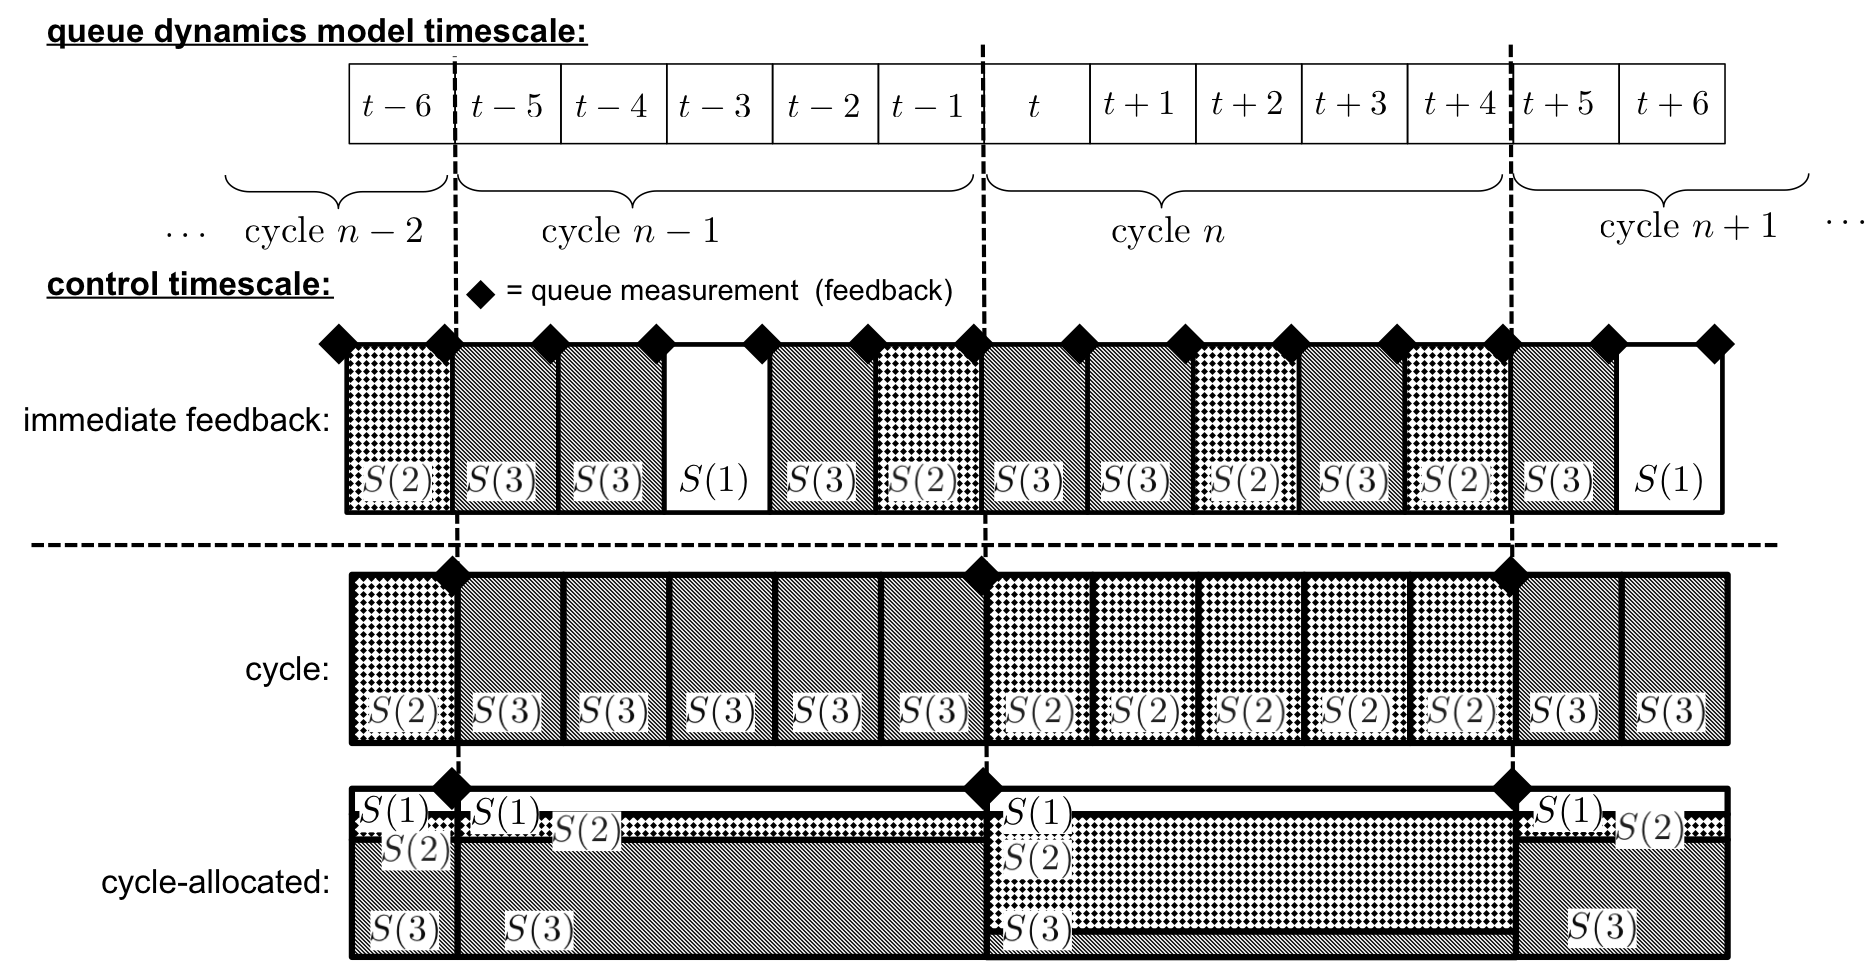
\includegraphics[width=\columnwidth]{./extensions_graphic.png}
%\caption{Extensions of max pressure modify the time scale of feedback and actuation. In this illustrations, consider three different feasible control actions represented by three degrees of shading. In the (original) immediate feedback formulation, measurements and control decisions are made at each model timestep; hence actuations can change as rapidly as queue states. \label{fig:variations}}
%\end{figure}
%
%


%% !TEX root = ./MParticle.tex
\section{Practical Constraints on the Controller} \label{sec:constraints}

Varaiya \cite{} assumes that the controller can be updated every time step. 
In real traffic systems, this is not possible. As a matter of fact, for hardware/technical reasons, one must keep the same control every $\tau$ time steps.
This can be seen as the fact that the dynamics are updated quicker than the control.

Also, Varaiya suppose that only one control matrix is chosen during the optimisation procedure, i.e. only one of the possible non conflicting phases is chosen.
This is not realistic in practice either, since each set of phases must be allocated a minimal (non nul) time.
In that case, instead of choosing the controller over a finite  set, a convex combination of control matrices is chosen. 
The coefficient $\lambda_{S}$ chosen for each phase $S$ represents the fraction (between 0 and 1) of the physical time allocated.
To ensure that each phase is guaranteed a minimum time, we want to constraint the coefficients of the convex combination to be all larger than $\kappa$.
(It is pretty straightforward to notice that $\kappa$ must satisfy the following: 

$$
\kappa | \text{set of non conflicting phases } | < 1
$$

We therefore reformulate the controller so that instead of a single phase being chosen for actuation at every model step, all feasible phases are actuated in parallel during the time step at a proportionally reduced rate. The control output will no longer be a binary matrix, but rather will be a \emph{relaxed} control matrix $S^r (t)$ which is a convex combination of all elements in the set of feasible control phases $U$. Each element $S^r (t)(i,j) \in [0,1]$ will represent fraction of the flow capacity at time step $t$ that is allocated to movement $(i,j)$. 
% !TEX root = ./MParticle.tex
\section{Relaxation of the Max Pressure Controller. Stability of the new Controller} \label{sec:immediatefeedback}




%%%%%%%%%
%relaxation of the controller
%%%%%%%%%
 

%%%%%%%%%%%
%Physically, one could consider one model time step to represent an entire light cycle, during which each signal phase will be sequentially actuated for some proportional amount of the period. (Although this would suggest a serial division of the time period between independent phases rather than the parallel implementation that is represented here mathematically.) 
%%%%%%%%%%%


We reformulate the controller so as to fullfill those guarantees. 
Then we show that a similar stability result as the one shown by Varaiya holds (under some \emph{slightly} weaker conditions).
To fulfill the first condition, we allow the control to be a convex combination of the different possible control matrices.
For the second condition we consider a control that is not updated every time steps.
The final control that we choose is a combination of the two.







%%%%%%%%%%%%%%%%%%%%%%%%%%%
%distributed max pressure
%%%%%%%%%%%%%%%%%%%%%%%%%%%
 




\subsection*{Phase distribution within a cycle}
We next investigate how the max pressure controller must be altered to allow the minimum proportion constraints on each phase in the set of allowable phases $\mathcal U$.

Let $T$ be the cycle length satisfying \eqref{minTime} and $\kappa_S$ be the minimum proportion of the cycle which must be allocated to each $S\in U$. %By definition, our controller must therefore satisfy the following condition:
%\begin{equation}
%T = (\sum_{S \in \mathcal U } \lambda_{S})T+ L
%\end{equation}
The allocated max pressure controller selects a set of $\lambda_S$ that maximizes alleviated pressure under the following constraints:
\begin{itemize}
\item $\lambda_{S} \geq \kappa_S$ 
\item $f_{l}r_{l,m} < \sum_{S}\lambda_{S} c(l,m)S(l,m)$
\item $ \sum_{S} \lambda_{S} = 1 - \frac{L}{T}$
\end{itemize}
%We therefore formulate the following convex optimization problem: 
%\begin{equation*}
%\begin{aligned}
%& \underset{\lambda_{1},...,\lambda_{\vert U\vert}}{\text{maximize}}
%& & \displaystyle\displaystyle\sum_{l,m} w(l,m)(t)c(l,m)(\displaystyle\sum_{S \in \mathcal{U}}\lambda_{S}S(l,m))  \\
%& \text{subject to}
%& &  \lambda_{S} \geq \kappa_S \\
%&&& \displaystyle\sum_{S} \lambda_{S} \leq 1 - \dfrac{L}{T}
%\end{aligned}
%\end{equation*}
The desired controller is therefore determined by the solution to the following linear program: 
\begin{align} \nonumber
\{ \lambda^*_S \} = \; & \underset{\lambda_{1},...,\lambda_{\vert U\vert}}{ \arg \max} & & \sum_{S \in \mathcal{U}}\lambda_{S}\Big(\sum_{l,m} w(l,m)(t)c(l,m) S(l,m)\Big)  \\
\nonumber & \text{subject to}
\nonumber & &  \lambda_{S} \geq \kappa_s\\
&&&\sum_{S} \lambda_{S} \leq 1 - \tfrac{L}{T}  \label{distMP_LP}
\end{align}



The solution to \eqref{distMP_LP} selects coefficients $\{ \lambda_{S}^{*} \} $ which form a corresponding relaxed control
matrix \begin{equation} S^{r*} = \displaystyle\sum_{S \in \mathcal{U}}\lambda_{S}^{*}S\end{equation}




\subsection*{Cycle max pressure}

Cycle max pressure enables the control to act at a slower time scale than the queue dynamics, as would be the case in a practical traffic application. Suppose that we are given the model dynamics $X(t)$ as in \eqref{entrydynamics}-\eqref{internaldynamics}, but the controller $S^*(t)$ can only be updated every $\tau$ model time steps (or once per \emph{cycle}). The ``$\tau$-non updated'' control sequence is therefore composed of control matrices repeated for at least $\tau$ model time steps: for a fixed cycle size $\tau$ and integer $n$, 
\begin{align} \nonumber
S(n\tau&+1)  = S(n\tau +2) = \ldots = S((n+1)\tau ) = S^*(n\tau +1) \\
&=  \arg\max\{\gamma(S)(X(n\tau +1 )) \vert S \in U\}  
 \label{CYCLE_CONTROLLER}
\end{align}
Physically, the controller that maximizes the pressure at time step $n\tau + 1$ is continuously applied until time step $(n + 1)\tau$.

\subsection*{Relaxed Max Pressure Controller}

Let $\tau \in \mathbb{N}$ be fixed, the number of time steps between two actuation of the controller
$\forall n \in \mathbb{N}$, 

\begin{align} \nonumber
S(n\tau&+1)   = \ldots = S((n+1)\tau ) = S^*(n\tau +1) \\
&=  \arg\max\{\gamma(S)(X(n\tau +1 )) \vert S \in U\}  \\
& =  \underset{\lambda_{1},...,\lambda_{\vert U\vert}}{ \arg \max}  \sum_{S \in \mathcal{U}}\lambda_{S}\Big(\sum_{l,m} w(l,m)(t)c(l,m) S(l,m)\Big)  \\
\nonumber  & \text{subject to}\\
\nonumber  &  \lambda_{S} \geq \kappa_s\\
& \sum_{S} \lambda_{S} \leq 1 - \tfrac{L}{T}  \label{distMP_LP}\\
& = S^{r*} \\
&= \displaystyle\sum_{S \in \mathcal{U}}\lambda_{S}^{*}S
\end{align}


\subsection*{Minimum cycle time}
Consider that the length $T$ of the controller update time period (signal cycle) is not pre-defined. However, there is a known amount of \emph{lost time} $L$ per cycle during which no phases can be actuated to account for physical clearance of the intersection between actuated phases. Hence it must be the case that $T>L$.  We furthermore impose that each feasible phase has an associated minimum proportion constraint: phase $S$ must be actuated for at least $\lambda_S T$ seconds during any one cycle. We then want to determine the minimum control period or \emph{cycle length} for which a fixed demand flow can be served while the stated phase proportion constraints are satisfied. 

Unlike the previous case where we constrained our analysis to flows which could be served in average over an arbitrary long-term time horizon, here our proof of stability depends on the assumption that the average demand is served \textit{within a single cycle}. As suggested in \cite{MaxPressureStochastic}, we then pose the selection of a cycle length as a convex optimization problem with constraints applied to enforce the desired minimum phase proportions $\kappa$:
\begin{equation} \label{sum_lambda}
\begin{aligned}
& \underset{\lambda = (\lambda_{S})_{S}}{\text{minimize}}
& & \sum_{S\in U} \lambda_{S} \\
& \text{subject to}
& &  \lambda_{S} \geq \kappa_S\\
&&& f_{l}r(l,m) < \sum_{S}\lambda_{S} c(l,m)S(l,m)\\
%&&& \sum_{S} \lambda_{S} < 1
\end{aligned}
\end{equation}
where $\kappa_S \in [0,1] \; \forall S\in U$, and $\sum_S \kappa_S <1$. 
%
%This is an obvious extension of the the linear program for a single intersection proposed by Allsop \cite{Allsop} and an implicit version of the formulation of Wong and Yang \cite{Wong}

Let us denote $\Lambda^{*}$ to be the optimum of  \eqref{sum_lambda}. If $\Lambda^* > 1$, the demand is not feasible under the set of control constraints $\{\kappa_S\}$ for any length time step. If $\Lambda^* < 1$, then the flow is admissible for a time step of length 
\begin{equation} T > \frac{L}{1-\Lambda^*} \label{minTime} \end{equation} 
We can now use this lower bound to select an appropriate cycle length. 


\subsection*{$\tau$-admissible flows}
We first prove that this set of $\tau$-admissible flows (demands that can be accommodated using $\tau$-non updated sequences) is in fact the same set of flows that is admissible under typical updated control sequences, defined in equation \eqref{feasible_demand}. 

\noindent Define the following sets:
\begin{itemize}
\item $U$ is the set of admissible control matrices as in \eqref{feasible_demand},
\item $U_{\mathbb{N}}$ is the set of control sequences $\{S(1), S(2) \ldots S(t) \ldots |  S(\cdot) \in U\} $ where elements are applied at consecutive time steps,
\item $U_{\tau\mathbb{N}}$ is the set of control sequences $\{S(1), S(1), \ldots ,  S(\tau + 1),S(\tau + 1), \ldots , S(n\tau + 1),S(n\tau + 1), \ldots |  S(\cdot) \in U\} $ where controls are updated only once every $\tau$ steps,
\item $conv(U) = \Big\{\lim\inf_{T} \dfrac{1}{T}\sum_{t=1}^{T} S(t) | \{S(1), S(2), \ldots , \\ S(t), \ldots \}\in U_{\mathbb{N}} \Big\} $ 
\item $conv(U_\tau ) = \Big\{\lim\inf_{T} \dfrac{1}{T}\sum_{t=1}^{T} S(t) | \{S(1), S(1), \ldots, \\ S(\tau + 1),S(\tau + 1), \ldots\}\in U_{\tau\mathbb{N}} \Big\} $ 
\end{itemize}
Obviously, $conv(U_{\tau}) \subset conv(U)$. But we can also show that $conv(U) \subset conv(U_{\tau})$:  

\noindent Suppose $M \in conv(U)$, so $\exists \{ S(1) \ldots S(t) \ldots \}$ such that $M = \lim\inf_{T} \dfrac{1}{T}\sum_{t=1}^{T} S(t)$.
\begin{align*}
M &= \lim\inf_{T} \dfrac{1}{T}\sum_{t=1}^{T} S(t)= \lim\inf_{T} \dfrac{1}{\tau T}\sum_{t=1}^{\tau T}  \tilde{S}(t) \; \\ 
& \qquad \text{ with } \tilde{S} = \{S(1), \ldots, S(1), \ldots, S(t), \ldots, S(t), \ldots \} \\
&= \lim\inf_{T} \dfrac{1}{ T}\sum_{t=1}^{T}  \tilde{S}(t) \\
\end{align*}
Trivially, $\tilde{S }\in conv(U_\tau)$. Because $conv(U_{\tau})\subset conv(U)$ and $cont(U) \subset conv(U_{\tau})$, it must hold that $conv(U) = conv(U_{\tau})$.  This establishes Property \ref{equality_property}: 

\begin{Prop} \label{equality_property}
\begin{equation*} conv(U) = conv(U_{\tau}) \end{equation*}
\end{Prop}

This property implies that a $\tau$-non updated control sequence can accommodate the same set of flows as a control sequence updated at every time step. The equivalence becomes intuitive when one considers that our definition of feasible flows considers only the long-term average of demand and service rates: note that a $\tau$ control matrix in $\tilde S$ is simply the average of the corresponding $\tau$ matrices in $\overline S$, such that $M_{\tilde S} = M_{\overline S}$. Hence,
\begin{align}
f_{l} r(l,m) < c(l,m)M_{\overline{S} }(l,m) \implies \\ f_{l} r(l,m) < c(l,m)M_{\tilde{S} }(l,m). \nonumber
\end{align}
However, as we will show in the following sections, the bound on queue lengths when the cycle controller is applied will be larger than in the immediate feedback setting.
%, which immediately seems counterintuitive. However, note that our current model framework assumes infinite link buffer capacities. With the $\tau$-non updated controller, instantaneous link queues will be higher but the same \emph{long-term average} service rates can be achieved -- and thus by our definition, this flow can be equally accommodated by either controller type. 
%We have shown that the same flows are ``admissible'' when control sequences updated only every $\tau$ time steps as when they are updated every time step. 
%During a single time step, the average flow arriving at queue $(l,m)$ is $f_{l}r(l,m)$ and the maximum number of vehicles capable of leaving is $c(l,m) M(l,m)$. Similarly, the average flow arriving between time steps $t$ and $t+\tau$ is $\tau f_{l} r(l,m) $, and the number of vehicles capable of leaving is $\tau c(l,m) M(l,m)$. So if a flow is admissible using an updated control sequence $\overline S$%with average service $M_{\overline S}$
%, it can be similarly accommodated with a non-updated sequence $\tilde S$, where each consecutive set of






\subsection*{Stability of the new controller}



Here we extend the previous proof of stability of an immediate feedback max pressure controller to the case of our relaxed max pressure controller.
We begin by defining two sets we gonna use later.

Define $conv_{\kappa}$ as the set of convex combinations of control matrices with coefficients larger than $\kappa$:
\begin{equation}
conv_{\kappa} = \Big\{ \sum_{S}\lambda_{S}S \big| \; \lambda_S > \kappa_S \; \forall S\in U\Big\}
\end{equation}
Also define a set of reduced admissible demands $D_{\kappa}$ which can in average be served in a single cycle with a relaxed control matrix that maintains the minimum time allocation for a given cycle time (as in \eqref{sum_lambda}):
\begin{align} \nonumber
d \in D_{\kappa} \; & \text{iff} \; \exists \; S^r \in conv_{\kappa} \; \\ & \text{such that} \; f_{l}r(l,m) < c(l,m)S^r(l,m)
\label{admissible_relaxed}
\end{align} 

\vspace{0.5cm}


\begin{Thm}\label{stabRelaxMP}
The relaxed max pressure controller, defined above, updated every $\tau$ iterations stabilizes the network whenever the demand is within a set of feasible demands $D^{\kappa}$.
\end{Thm}

\begin{proof}



%
%\subsubsection*{Immediate feedback Max Pressure: proof of Theorem 3}
%% !TEX root = ./MParticle.tex
\label{app_oldproof}

Consider the expectation of the following function of queue state with perturbation 
\begin{equation} \label{delta_def}
\delta(t) = X(t+1) - X(t)
\end{equation}  
conditioned on the past queue state:
\begin{align}
\vert X(t+1) \vert^2  - \vert X(t)\vert^2 &= \vert X(t) + \delta (t) \vert^2 - \vert X(t)\vert^2 \\
\nonumber &= 2X(t)^{T}\delta(t) + \vert \delta(t)  \vert^2 \\
\nonumber &= 2\alpha(t) + \beta(t) 
\end{align}
with 
\begin{equation} \label{alpha_beta_defs}
\alpha(t)  = X(t)^{T}\delta(t)  \text{   \; and \;  }\beta(t) = \vert \delta (t) \vert^{2}
\end{equation}
We continue by addressing bounds on $\beta$ and $\alpha$ separately. 

\subsection*{Bound on $\beta(t) = \vert \delta (t)\vert^{2}$}
Define $\overline{C}$ as the maximum realized saturation flow and $\overline{d}$ as the maximum possible value of the demand vector. 
If $l \in \entrylinks$ and $m \in Out(l)$,
\begin{align} \nonumber
\big| \delta(l,m)(t)  \big| &= \bigg| -[C(l,m)(t+1)S(l,m)(t) \wedge x(l,m)(t)]  \\ \nonumber
&\qquad \qquad + D(l,m)(t+1) \bigg| \\
& \leq \max\left\{  \overline{C}(l,m) , \overline d (l,m) \right\} \label{deltabound1}
\end{align}
where $D(l,m)(t)  = D(l) (t) R(l,m)(t)$ with $D(l)(t)$ defined as the realized demand on link $l$ at time $t$. 
This is because we know that both $C(l,m)(t+1)S(l,m)(t) \wedge x(l,m)(t)$ and $D(l,m)(t+1)$ are non-negative, so the absolute value of their difference must be less than either of the two quantities individually. 

Similarly, if $l \in \linkset\backslash\entrylinks$ and $m \in Out(l)$:
\begin{align} \nonumber  
\big | \delta(l,&m) (t)  \big |  = \\ \label{deltabound}
 & \bigg\vert-\big[C(l,m)(t+1)S(l,m)(t) \wedge x(l,m)(t)\big]  \\  \nonumber
 & + \sum_{k}\big[C(k,l)(t+1)S(k,l)(t) \wedge x(k,l)(t)\big] R(l,m)(t+1)\bigg\vert  \\
& \leq \max\left\{  \overline{C}(l,m) , \sum_{k} \overline{C}(k,l) \right\} \label{deltabound2}
\end{align}

If we define $B$ as the maximum of all of the quantities $\left\{ \overline{C}(l,m), \sum_{k} \overline{C}(k,l),  \overline d (l,m) \right\}$ and $N$ as the number of queues in the network, we can derive a bound for $\beta$ which depends on only $B$ and $N$: 
\begin{equation}\label{betabound}
\beta(t)  = \big| \delta(t) \big|^2 \leq NB^2 
\end{equation}

Note that because these bounds hold for any $S(l,m)(t) \in [0,1]$, the bound on $\beta$ presented here can easily be extended to 
any convex combination of control matrices; hence it is still valid in our modified controllers, as shown later in this article.
%Such an extension is not as trivial with the $\alpha$ term. 

\subsection*{Bound on $\alpha (t) = X(t)^{T}\delta(t) $}
The term $\alpha$ in \eqref{alpha_beta_defs} is explicitly defined in terms of queue state $X(t)$ as follows: 

\begin{align} \nonumber 
 \alpha (t)  &=  X(t)^{T}\left[X(t+1) - X(t)\right] \\ \nonumber
 &=  \sum_{l \in \linkset \backslash \entrylinks ,m}\sum_{k}\left[ C(k,l)(t+1)S(k,l)(t)\wedge x(k,l)(t)\right]\\ \nonumber
&\qquad \qquad  \quad \cdot R(l,m)(t+1)x(l,m)(t) \\ \nonumber
&  \qquad \qquad -  \sum_{l \in \linkset,m}\left[ C(l,m)(t+1)S(l,m)(t)\wedge x(l,m)(t)\right] \\ \nonumber
&\qquad \qquad-\sum_{l \in \entrylinks ,m} d(l,m)(t+1)x(l,m)(t)\\ \nonumber
&= \sum_{l \in \linkset,m}\big[C(l,m)(t+1)S(l,m)(t)\wedge x(l,m)(t)\big] \\ \nonumber 
& \qquad \qquad \cdot \Big(-x(l,m)(t)+  \sum_{p}R(m,p)(t+1)x(m,p)(t)\Big) \\  
 & \qquad \qquad + \sum_{l \in \entrylinks,m} d(l,m)(t+1)x(l,m)(t)  
 \label{alpha_explicit}
\end{align}
Note that only the expectation of these terms appear in equation \eqref{stability_sufficient}, so we are interested in $\mathbb{E}\{\alpha(t) | X(t)\}$. We therefore make the following observation: because $R(m,p)(t+1)$ is independent of $C(l,m)(t+1)$ and $X(t)$, 
\begin{align*}
\nonumber \expectation{&\big[C(l,m)(t+1)S(l,m)(t)\wedge x(l,m)(t)\big] \\
\nonumber & \qquad \quad  \;   \cdot R(m,p)(t+1)x(m,p)(t) \big| X(t)}  \\
\nonumber & = \expectation{\big[C(l,m)(t+1)S(l,m)(t)\wedge x(l,m)(t)\big]  \big| X(t)} \\
\nonumber & \qquad \quad  \; \cdot r(m,p)(t+1)x(m,p)(t)
\end{align*}

\vspace{0.5cm}

Also, the expectation of demand $d(l,m)$ is equal to the measured demand $d_{l}$ on link $l$, times the relevant expected split ratio $r(l,m)$. 
Hence the desired expectation of \eqref{alpha_explicit} can be expressed as
\begin{align} 
\nonumber \mathbb{E} & \{\alpha (t) | X(t)\}= \\
\nonumber & \sum_{l \in \linkset,m} \expectation{ \big[C(l,m)(t+1)S(l,m)(t)\wedge x(l,m)(t)\big]\big| X(t)}\\
\nonumber & \qquad \quad  \;   \cdot \Big(-x(l,m)(t) + \sum_{p}r(m,p)(t+1)x(m,p)(t)\Big) \\
 \nonumber &\qquad + \sum_{l \in \entrylinks,m} d_l r(l,m) x(l,m)(t)  \\
 \nonumber =& \sum_{l \in \entrylinks,m} d_l r(l,m) x(l,m)(t) \\
\nonumber &- \sum_{l \in \linkset,m} \expectation{ \big[C(l,m)(t+1)S(l,m)(t)\wedge x(l,m)(t)\big] \big| X(t)} \\  
\label{Ea} &\qquad \qquad \cdot w(l,m)(t)
\end{align}
where $w(l,m)(t) = w(l,m)(X(t))$ is the weight of a link as defined in \eqref{linkweight}. 
We also can include the following relation: 
\begin{align*}
\sum_{l \in \linkset,m} f_l &r(l,m) w(l,m)(t) \\ 
& = \sum_{l \in \linkset,m} f_l r(l,m) \left[ x(l,m) - \sum_p r(m,p)x(m,p)(t) \right] \\
& = \sum_{l \in \linkset,m} f_l r(l,m)x(l,m)(t) \\
&\qquad \qquad - \sum_m  \left[ \sum_{l\in\linkset} f_l r(l,m) \sum_p r(m,p)x(m,p)(t) \right] \\
& = \sum_{l \in \linkset,m} f_l r(l,m)x(l,m)(t)\\
&\qquad \qquad  - \sum_{m\in \linkset \backslash \entrylinks, p}   f_m r(m,p)x(m,p)(t) \\ 
& =  \sum_{l \in \entrylinks,m} d_l r(l,m)x(l,m)(t)
\end{align*}
So \eqref{Ea} is further simplified to: 
\begin{align} \label{expected_short}
 & \mathbb{E}\{\alpha (t) | X(t)\} = \sum_{l \in \linkset,m} \bigg[ f_l r(l,m)  \\
 \nonumber  & - \expectation{ \big[C(l,m)(t+1)S(l,m)(t)\wedge x(l,m)(t)\big] \big| X(t)}  \bigg] w(l,m)(t)  \\  
 & \qquad \qquad = \alpha_1 (t) + \alpha_2 (t) \nonumber
\end{align}
with 
\begin{align} \label{a1_def}
\alpha_1 (t) &=  \sum_{l \in \linkset,m} \left[ f_l r(l,m) - c(l,m)S(l,m)(t) \right] w(l,m)(t)   \\
\nonumber \text{ and }&  \\ 
 \alpha_2 (t) & =  \sum_{l \in \linkset,m} \Big[ c(l,m)- \\ \nonumber
\expectation{ \big[C & (l,m)(t+1)\wedge x(l,m)(t)\big] \big| X(t) }  \Big] S(l,m)(t)w(l,m)(t)  
\end{align}
These $\alpha_{\{1,2\}}$ are derived by first including in \eqref{expected_short} the $0$-valued term $[c(l,m)S(l,m)(t)w(l,m)(t) - c(l,m)S(l,m)(t)w(l,m)(t)]$, and then assuming that $S(l,m)(t) \in \{0,1\}$ (hence it can be brought outside of the internal min function in $\alpha_2$ without changing the ultimate result). %The later assumption does not hold in our modified controllers. 
\begin{Lem} \label{alpha2bound}
For all $l$, $m$, $t$, 
\begin{equation} 
\alpha_2 (t) \leq \sum_{l \in \linkset,m} c(l,m)\overline{C} (l,m)
\end{equation}
where $\overline{C} (l,m)$ is the maximum value of the random service rate $C(l,m)(t)$. 
\end{Lem}
\underline{Proof of Lemma \ref{alpha2bound}:} \\
By Jensen's inequality, 
\begin{align*}
\expectation{C(l,m)(t+1) & \wedge x(l,m)(t) \big| X(t)} \\
& \leq \expectation{C(l,m)(t+1) \big| X(t)}  \wedge x(l,m)(t) \\
&= c(l,m)\wedge x(l,m)(t) \\ 
&\leq c(l,m)
\end{align*}
 Furthermore, we know that the term 
$ \left[ c(l,m)- \expectation{ \big[C(l,m)(t+1)\wedge x(l,m)(t)\big] \big| X(t) }  \right] $
is non-negative, and only equal to $0$ when $x(l,m)(t)>\overline C (l,m)$. 
Using these relations and the observations that $w(l,m)(t) \leq x(l,m)(t)$ and $S(l,m)(t)\in \{0,1\}$, the following must hold 
\begin{align*}
\alpha_2 (t) & = \sum_{l \in \linkset,m} \left[ c(l,m)- \expectation{ \big[C(l,m)(t+1)\wedge x(l,m)(t)\big] \big| X(t) }  \right] \\ &\qquad \qquad \qquad \cdot S(l,m)(t)w(l,m)(t) \\
& \leq \sum_{l \in \linkset,m} \left[ c(l,m)- \expectation{ \big[C(l,m)(t+1)\wedge x(l,m)(t)\big] \big| X(t) }  \right] \\ &\qquad \qquad \qquad \cdot S(l,m)(t)x(l,m)(t)   \\
& \leq \sum_{l \in \linkset,m} c(l,m) \overline{C}(l,m)
 \end{align*}



 \begin{Lem} \label{alpha1bound}
If the immediate feedback max pressure control policy $u^*$ is applied and the demand $d$ is in the set of feasible demands $D^o$, then there exists an $\varepsilon>0$, $\eta>0$ such that 
\begin{equation} 
\alpha_1(t)  \leq -\varepsilon \eta \big| X(t)\big| 
\end{equation}
\end{Lem}
\underline{Proof of Lemma \ref{alpha1bound}:} \\
Applying the definition of immediate feedback max pressure control in \eqref{original_MP} as $S^*$, 
\begin{align*}
\sum_{l,m} S^* (l,m)&(t) c(l,m) w(l,m)(t) \\
&= \max_{S\in U} \sum_{l,m} S(l,m)c(l,m)w(l,m)(t) \\
&= \max_{M\in co(U)} \sum_{l,m} M(l,m)c(l,m)w(l,m)(t)
\end{align*}
As in \eqref{feasible_demand}, since $d\in D^0$, there exists an $\varepsilon > 0$ and $M^+$ such that $C(l,m)M^+(l,m) > f_l r(l,m) + \varepsilon \; \forall (l,m)$. Logically, any $M'$ such that $0\leq M' \leq M^+$ (component-wise) must also be in $co(U)$. Therefore we choose a $M' < M^+$ such that 
\begin{equation} \label{epsDef}
M'(l,m) c(l,m) = \begin{cases} 
f_l r(l,m) + \varepsilon  & \text{ if } w(l,m)>0 \\
0 & \text{ if }w(l,m)\leq 0
\end{cases}
\end{equation} 
 Then
 \begin{align} %\label{alpha1_intermediate}
\nonumber  \alpha_1 (t) & =  \sum_{l \in \linkset,m} \left[ f_l r(l,m) - c(l,m)S^*(l,m)(t) \right] w(l,m)(t) \\
 \nonumber & \leq \sum_{l \in \linkset,m} \left[ f_l r(l,m) - M'(l,m)c(l,m) \right] w(l,m)(t) \\
\nonumber & = -\varepsilon \sum_{l \in \linkset,m} \max\{w(l,m)(t),0\} \\
\nonumber & \qquad \qquad +  \sum_{l \in \linkset,m}  f_l r(l,m)  \min\{ w(l,m)(t),0\} \\
& \leq -\varepsilon \sum_{l \in \linkset,m}  \left| w(l,m) (t) \right| \label{alpha1_w}
\end{align}
Notice that $w(l,m)(X(t))$ is a linear, invertible function of the array $X(t)$, and therefore there exists a $\eta >0$ such that $\sum_{l,m} | w(l,m) (X(t)) | \geq \eta |X(t)|$. Substituting this expression into \eqref{alpha1_w} defines a bound on $\alpha_1$ (t): 
\begin{equation} \label{a1_bound_eq}
\alpha_1(t) \leq -\varepsilon \eta \left| X(t ) \right|
\end{equation}
Combining the results of Lemmas \ref{alpha2bound} and \ref{alpha1bound} generates the desired bound on $\expectation{\alpha (t) | X(t)}$:
\begin{equation}\label{alphabound}
\expectation{\alpha(t) | X(t)} \leq -\varepsilon \eta \left| X(t ) \right| + \sum_{l \in \linkset,m} c(l,m)\overline{C} (l,m)
\end{equation}

\subsection*{Explicit bound on queues, immediate feedback MP}

Combining \eqref{alphabound} and \eqref{betabound}, we obtain
\begin{align}
\expectation{&|X(t+1)|^{2} - |X(t)|^{2}  |   X(t)} = \expectation{2\alpha(t) + \beta(t)} \nonumber \\
&<  -2\varepsilon \eta \left| X(t ) \right| + 2 \sum_{l \in \linkset,m} [c(l,m)\overline{C} (l,m) ]+ NB^{2}
\end{align}
where $N$ is the number of links in the network and $B=\max\left\{ \overline{C}(l,m), \sum_{k} \overline{C}(k,l),  \overline d (l,m) \right\}$. 
For simplicity, we combine all constant additive terms to define a new constant $K$:
\begin{align}\label{constCalc}
K = 2 \displaystyle\sum_{l,m} & c(l,m) \overline{C}(l,m) \\
\nonumber & + N \displaystyle\sum_{l,m} \max\left\{ \overline{C}(l,m), \sum_{k} \overline{C}(k,l),  \overline d (l,m) \right\}^2
\end{align}
So
\begin{equation}\label{stabBasic}
\expectation{|X(t+1)|^{2} - |X(t)|^{2}  |   X(t)} < -2\varepsilon \eta \left| X(t ) \right| + K
\end{equation}
%Therefore we have an inequality of the form
%\begin{equation}\label{stabBasic}
%\expectation{|X(t+1)|^{2} - |X(t)|^{2}  |   X(t)} < -\varepsilon \eta \left| X(t ) \right| + K
%\end{equation}
%where 
%\begin{equation}\label{constCalc}
%K = 2\displaystyle\sum_{l,m} c(l,m) \overline{C}(l,m) + \displaystyle\sum_{l,m} \max[\overline{C}(l,m),\sum_{k}\overline{C}(k,l)]^2
%\end{equation}
This is sufficient to show stability as previously defined.

%%%%%%%%
%END: Original proof
%%%%%%%%

%\subsection*{Comments for the extensions of the proof}
%
%To sum things up
%
%\begin{align*}
%\mathbb{E}[\vert X(t + 1) \vert - \vert X(t) \vert  \vert X(t)] &= 2\alpha(t) + \beta(t)\\
%&= 2\alpha_{1}(t) + 2\alpha_{2}(t) + \beta(t)\\
%&< 2\alpha_{1} + K
%\end{align*}
%
%since $\alpha_{2}(t)$ and $\beta(t)$ are bounded for any binary or relaxed controller.
%
%Therefore, if we manage to show a property such as 
%
%\begin{equation}
%\sum_{l,m} (f_{l}r(l,m) - c(l,m)S(l,m))w(l,m) < - \varepsilon \vert  X(t) \vert 
%\end{equation}
%
%for the controller, then stability instantanely follows.


\subsubsection*{Allocated Max Pressure: proof of Theorem 6}
% !TEX root = ./MParticle_resubmit.tex
\label{distributedproof}

%%%%%%%%%%%%%%%%%%%%%%%%%%%%%%%%%%%%%%%%%%%%%%%%%%%%%%%%%%%

Consider the expectation of the following function of queue state with perturbation 
\begin{equation} \label{delta_def}
\delta(t) = X(t+1) - X(t)
\end{equation}  
conditioned on the past queue state:
\begin{align}
\vert X(t+1) \vert^2  - \vert X(t)\vert^2 &= \vert X(t) + \delta (t) \vert^2 - \vert X(t)\vert^2 \\
\nonumber &= 2X(t)^{T}\delta(t) + \vert \delta(t)  \vert^2 \\
\nonumber &= 2\alpha(t) + \beta(t) 
\end{align}
\begin{equation} \label{alpha_beta_defs}
\text{with \quad} \alpha(t)  = X(t)^{T}\delta(t)  \text{   \; and \;  }\beta(t) = \vert \delta (t) \vert^{2}
\end{equation}
We continue by addressing bounds on $\beta$ and $\alpha$ separately. 
\subsection*{Bound on $\beta(t) = \vert \delta (t)\vert^{2}$}
%Define $\overline{C}$ as the maximum realized saturation flow and $\overline{d}$ as the maximum possible value of the demand vector. 
%If $l \in \entrylinks$ and $m \in Out(l)$,
%\begin{align} \nonumber
%\big| \delta(l,m)(t)  \big| &= \bigg| -[C(l,m)(t+1)S(l,m)(t) \wedge x(l,m)(t)]  \\ \nonumber
%&\qquad \qquad + D(l,m)(t+1) \bigg| \\
%& \leq \max\left\{  \overline{C}(l,m) , \overline d (l,m) \right\} \label{deltabound1}
%\end{align}
%where $D(l,m)(t)  = D(l) (t) R(l,m)(t)$ with $D(l)(t)$ defined as the realized demand on link $l$ at time $t$. 
%This is because we know that both $C(l,m)(t+1)S(l,m)(t) \wedge x(l,m)(t)$ and $D(l,m)(t+1)$ are non-negative, so the absolute value of their difference must be less than either of the two quantities individually. 
%
%Similarly, if $l \in \linkset\backslash\entrylinks$ and $m \in Out(l)$:
%\begin{align} \nonumber  
%\big | \delta(l,&m) (t)  \big |  = \\ \label{deltabound}
% & \bigg\vert-\big[C(l,m)(t+1)S(l,m)(t) \wedge x(l,m)(t)\big]  \\  \nonumber
% & + \sum_{k}\big[C(k,l)(t+1)S(k,l)(t) \wedge x(k,l)(t)\big] R(l,m)(t+1)\bigg\vert  \\
%& \leq \max\left\{  \overline{C}(l,m) , \sum_{k} \overline{C}(k,l) \right\} \label{deltabound2}
%\end{align}
If we define $B$ as the maximum of all of the quantities $\left\{ \overline{C}(l,m), \sum_{k} \overline{C}(k,l),  \overline d (l,m) \right\}$ and $N$ as the number of queues in the network, we can derive a bound for $\beta$ which depends on only $B$ and $N$: 
\begin{equation}\label{betabound}
\beta(t)  = \big| \delta(t) \big|^2 \leq NB^2 
\end{equation}
The proof of this bound is exactly the same as in \cite{MaxPressureStochastic}, and will therefore not be repeated here. However, note that because these bounds hold for any $S(l,m)(t) \in [0,1]$, this bound on $\beta$ is trivially extended to any convex combination of control matrices; hence it is still valid in our relaxed controllers {\color{red}(as will be shown later in this article)}.

\subsection*{Bound on $\alpha (t) = X(t)^{T}\delta(t) $}
%The term $\alpha$ in \eqref{alpha_beta_defs} is explicitly defined in terms of queue state $X(t)$ as follows: 
%\begin{small}
%\begin{align} \nonumber 
% \alpha (t)  &=  X(t)^{T}\left[X(t+1) - X(t)\right] \\ \nonumber
% &=  \sum_{l \in \linkset \backslash \entrylinks ,m}\sum_{k}\left[ C(k,l)(t+1)S(k,l)(t)\wedge x(k,l)(t)\right]\\ \nonumber
%&\qquad \qquad  \qquad \qquad  \qquad  \cdot R(l,m)(t+1)x(l,m)(t) \\ \nonumber
%&  \qquad \qquad -  \sum_{l \in \linkset,m}\left[ C(l,m)(t+1)S(l,m)(t)\wedge x(l,m)(t)\right] \\ \nonumber
%&\qquad \qquad-\sum_{l \in \entrylinks ,m} d(l,m)(t+1)x(l,m)(t)\\ \nonumber
%&= \sum_{l \in \linkset,m}\big[C(l,m)(t+1)S(l,m)(t)\wedge x(l,m)(t)\big] \\ \nonumber 
%& \qquad \qquad \cdot \Big(-x(l,m)(t)+  \sum_{p}R(m,p)(t+1)x(m,p)(t)\Big) \\  
% & \qquad \qquad + \sum_{l \in \entrylinks,m} d(l,m)(t+1)x(l,m)(t)  
% \label{alpha_explicit}
%\end{align}
%\end{small}
%{\color{red}Note that only the expectation of these terms appear in equation \eqref{stability_sufficient}, so we are interested in $\mathbb{E}\{\alpha(t) | X(t)\}$. } We therefore make the following observation: because $R(m,p)(t+1)$ is independent of $C(l,m)(t+1)$ and $X(t)$, 
%\begin{align*}
%\nonumber \expectation{&\big[C(l,m)(t+1)S(l,m)(t)\wedge x(l,m)(t)\big] \\
%\nonumber & \qquad \quad  \;   \cdot R(m,p)(t+1)x(m,p)(t) \big| X(t)}  \\
%\nonumber & = \expectation{\big[C(l,m)(t+1)S(l,m)(t)\wedge x(l,m)(t)\big]  \big| X(t)} \\
%\nonumber & \qquad \quad  \; \cdot r(m,p)(t+1)x(m,p)(t)
%\end{align*}
%Also, the expectation of demand $d(l,m)$ is equal to the measured demand $d_{l}$ on link $l$, times the relevant expected split ratio $r(l,m)$. 
%Hence the desired expectation of \eqref{alpha_explicit} can be expressed as
%%\begin{small}
%\begin{align*} 
%\nonumber \mathbb{E} & \{\alpha (t) | X(t)\}= \sum_{l \in \entrylinks,m} d_l r(l,m) x(l,m)(t)  \\
%\nonumber & + \sum_{l \in \linkset,m} \expectation{ \big[C(l,m)(t+1)S(l,m)(t)\wedge x(l,m)(t)\big]\big| X(t)}\\
%\nonumber & \qquad \qquad    \cdot \Big(-x(l,m)(t) + \sum_{p}r(m,p)(t+1)x(m,p)(t)\Big) 
% \end{align*}
% \begin{align}
% \label{Ea} = \sum_{l \in \entrylinks,m} &d_l r(l,m) x(l,m)(t)  - \sum_{l \in \linkset,m} w(l,m)(t) \; \cdot  \\
%\nonumber & \expectation{ \big[C(l,m)(t+1)S(l,m)(t)\wedge x(l,m)(t)\big] \big| X(t)}
%\end{align}
%%\end{small} 
%where $w(l,m)(t) = w(l,m)(X(t))$ is the weight of a link as defined in \eqref{linkweight}. 
%We also can include the following relation: 
%\begin{align*}
%\sum_{l \in \linkset,m} f_l &r(l,m) w(l,m)(t) \\ 
%& = \sum_{l \in \linkset,m} f_l r(l,m) \left[ x(l,m) - \sum_p r(m,p)x(m,p)(t) \right] \\
%& = \sum_{l \in \linkset,m} f_l r(l,m)x(l,m)(t) \\
%&\qquad \quad \; - \sum_m  \left[ \sum_{l\in\linkset} f_l r(l,m) \sum_p r(m,p)x(m,p)(t) \right] \\
%& = \sum_{l \in \linkset,m} f_l r(l,m)x(l,m)(t)\\
%&\qquad \qquad  - \sum_{m\in \linkset \backslash \entrylinks, p}   f_m r(m,p)x(m,p)(t) \\ 
%& =  \sum_{l \in \entrylinks,m} d_l r(l,m)x(l,m)(t)
%\end{align*}
Again following \eqref{MaxPressureStochastic}, we define the following sub-terms:
\begin{small}
\begin{align} \label{expected_short}
 & \mathbb{E}\{\alpha (t) | X(t)\} = \sum_{l \in \linkset,m} w(l,m)(t) \; \cdot   \\
 \nonumber  & \bigg[ f_l r(l,m) - \expectation{ \big[C(l,m)(t+1)S(l,m)(t)\wedge x(l,m)(t)\big] \big| X(t)}  \bigg]   \\  
 & \qquad \qquad = \alpha_1 (t) + \alpha_2 (t) \nonumber
\end{align}
\end{small}
with 
\begin{small}
\begin{align} \label{a1_def}
\alpha_1 (t) &=  \sum_{l \in \linkset,m} \left[ f_l r(l,m) - c(l,m)S(l,m)(t) \right] w(l,m)(t)   \\
\nonumber \text{ and }&  \\  \nonumber
 \alpha_2 (t) & =  \sum_{l \in \linkset,m}S(l,m)(t)w(l,m)(t)  \; \cdot   \\ 
&\Big[ c(l,m)- \expectation{ \big[C  (l,m)(t+1)\wedge x(l,m)(t)\big] \big| X(t) }  \Big]  
\end{align}
\end{small}
%These $\alpha_{\{1,2\}}$ are derived by first including in \eqref{expected_short} the $0$-valued term $[c(l,m)S(l,m)(t)w(l,m)(t) - c(l,m)S(l,m)(t)w(l,m)(t)]$, and then assuming that $S(l,m)(t) \in \{0,1\}$ (hence it can be brought outside of the internal min function in $\alpha_2$ without changing the ultimate result). %The later assumption does not hold in our modified controllers. 
\begin{Lem} \label{alpha2bound}
For all $l$, $m$, $t$, 
\begin{equation} 
\alpha_2 (t) \leq \sum_{l \in \linkset,m} c(l,m)\overline{C} (l,m)
\end{equation}
where $\overline{C} (l,m)$ is the maximum value of the random service rate $C(l,m)(t)$. 
\end{Lem}
\underline{Proof of Lemma \ref{alpha2bound}:} \\
By Jensen's inequality, 
\begin{align*}
\expectation{C(l,m)(t+1) & \wedge x(l,m)(t) \big| X(t)} \\
& \leq \expectation{C(l,m)(t+1) \big| X(t)}  \wedge x(l,m)(t) \\
&= c(l,m)\wedge x(l,m)(t) \\ 
&\leq c(l,m)
\end{align*}
 Furthermore, we know that the term 
$ \left[ c(l,m)- \expectation{ \big[C(l,m)(t+1)\wedge x(l,m)(t)\big] \big| X(t) }  \right] $
is non- negative, and only equal to $0$ when $x(l,m)(t)>\overline C (l,m)$. 
Using these relations and the observations that $w(l,m)(t) \leq x(l,m)(t)$ and $S(l,m)(t)\in [0,1]$, the following must hold 
\begin{align*}
\alpha_2 (t) & =  \sum_{l \in \linkset,m}  S(l,m)(t)w(l,m)(t) \; \cdot  \\
 & \qquad  \left[ c(l,m)- \expectation{ \big[C(l,m)(t+1)\wedge x(l,m)(t)\big] \big| X(t) }  \right] \\
& \leq \sum_{l \in \linkset,m} S(l,m)(t)x(l,m)(t) \; \cdot \\ 
& \qquad \left[ c(l,m)- \expectation{ \big[C(l,m)(t+1)\wedge x(l,m)(t)\big] \big| X(t) }  \right] \\
& \leq \sum_{l \in \linkset,m} c(l,m) \overline{C}(l,m)
 \end{align*}



 \begin{Lem} \label{alpha1bound}
If the relaxed max pressure control policy $u^*$ is applied at time step $t$ and the demand $d$ is in the set of feasible demands $D^\kappa$, then there exists an $\varepsilon>0$, $\eta>0$ such that 
\begin{equation} 
\alpha_1(t)  \leq -\varepsilon \eta \big| X(t)\big| 
\end{equation}
\end{Lem}
\underline{Proof of Lemma \ref{alpha1bound}:} \\
Consider the relaxed control matrix $S^{r*}$ specified by \eqref{distMP_LP}. By construction, it must be true that $ \forall S^r \in conv_{\kappa}$, 
\begin{align} \nonumber
\sum_{l,m}c(l,m)& w(l,m)(X(t))S^r (l,m) \\
&\leq \sum_{l,m}c(l,m)w(l,m)(X(t))S^{r*}(l,m) 
\end{align}
with equality only if $S^r = S^{r*}$. 
Therefore $\forall S^r \neq S^{r*}$,
\begin{align} \nonumber
 \sum_{l,m}&\big[f_{l}r(l,m) - c(l,m)S^{r*}(l,m)(t)\big]w(l,m)(X(t)) \\
&<   \sum_{l,m}\big[f_{l}r(l,m) - c(l,m)S^r(l,m)\big]w(l,m)(X(t))
\end{align}
If the demand flow is admissible according to \eqref{admissible_relaxed}, then 
$\exists \Sigma \in conv_{\kappa}$ such that 
\begin{equation} \nonumber
c(l,m)\Sigma(l,m) = \begin{cases}
        f_{l}r(l,m) + \varepsilon & \text{ if } w(l,m)(X(t)) > 0 \\
        0 & \text{ otherwise}
    \end{cases}
\end{equation}
{\color{red} Hence following the same logic as in \eqref{alpha1_w}, }
\begin{align} \nonumber
 \sum_{l,m}&\big[f_{l}r(l,m) -  c(l,m)S^{r*}(l,m)(t)\big] w(l,m)(X(t))  \\ \nonumber
&  < -\varepsilon \sum_{l \in \linkset,m} \max\{w(l,m)(X(t)) ,0\} \\
&\qquad +  \sum_{l \in \linkset,m}  f_l r(l,m)  \min\{ w(l,m)(X(t)) ,0\}
\end{align}
We assume that by our choice of $\sigma(l,m)$, $f_{l}r(l,m) > \varepsilon$ (omitting the cases where $r(l,m) = 0$). Therefore:
\begin{align}\nonumber
\sum_{l,m}\big[ f_{l}r(l,m) & - c(l,m)S^{r*}(l,m)(t)\big]w(l,m)(X(t)) \\
&< -\varepsilon \displaystyle\sum_{l,m} x(l,m)(t)
\end{align}

\subsection*{Explicit bound on queues, immediate feedback MP}
{\color{red} Combining \eqref{alphabound} and \eqref{betabound}, we obtain}
\begin{align}
\expectation{&|X(t+1)|^{2} - |X(t)|^{2}  |   X(t)} = \expectation{2\alpha(t) + \beta(t)} \nonumber \\
&<  -2\varepsilon \eta \left| X(t ) \right| + 2 \sum_{l \in \linkset,m} [c(l,m)\overline{C} (l,m) ]+ NB^{2}
\end{align}
where $N$ is the number of links in the network and $B=\max\left\{ \overline{C}(l,m), \sum_{k} \overline{C}(k,l),  \overline d (l,m) \right\}$. 
For simplicity, we combine all constant additive terms to define a new constant $K$:
\begin{align}\label{constCalc}
K = 2 \displaystyle\sum_{l,m} & c(l,m) \overline{C}(l,m) \\
\nonumber & + N \displaystyle\sum_{l,m} \max\left\{ \overline{C}(l,m), \sum_{k} \overline{C}(k,l),  \overline d (l,m) \right\}^2
\end{align}
So, when the control is updated at time $t$:
\begin{equation}\label{stabBasic}
\expectation{|X(t+1)|^{2} - |X(t)|^{2}  |   X(t)} < -2\varepsilon \eta \left| X(t ) \right| + K
\end{equation}
%Therefore we have an inequality of the form
%\begin{equation}\label{stabBasic}
%\expectation{|X(t+1)|^{2} - |X(t)|^{2}  |   X(t)} < -\varepsilon \eta \left| X(t ) \right| + K
%\end{equation}
%where 
%\begin{equation}\label{constCalc}
%K = 2\displaystyle\sum_{l,m} c(l,m) \overline{C}(l,m) + \displaystyle\sum_{l,m} \max[\overline{C}(l,m),\sum_{k}\overline{C}(k,l)]^2
%\end{equation}




%%%%%%%%%%%%%%%%%%%%%%%%%%%%%%%%%%%%%%%%%%%%%%%%%%%%%%%%%%%





%Consider the relaxed control matrix $S^{r*}$ specified by \eqref{distMP_LP}. By construction, it must be true that $ \forall S^r \in conv_{\kappa}$, 
%\begin{align} \nonumber
%\sum_{l,m}c(l,m)& w(l,m)(X(t))S^r (l,m) \\
%&\leq \sum_{l,m}c(l,m)w(l,m)(X(t))S^{r*}(l,m) 
%\end{align}
%with equality only if $S^r = S^{r*}$. 
%Therefore $\forall S^r \neq S^{r*}$,
%\begin{align} \nonumber
% \sum_{l,m}&\big[f_{l}r(l,m) - c(l,m)S^{r*}(l,m)(t)\big]w(l,m)(X(t)) \\
%&<   \sum_{l,m}\big[f_{l}r(l,m) - c(l,m)S^r(l,m)\big]w(l,m)(X(t))
%\end{align}
%If the demand flow is admissible according to \eqref{admissible_relaxed}, then 
%$\exists \Sigma \in conv_{\kappa}$ such that 
%\begin{equation} \nonumber
%c(l,m)\Sigma(l,m) = \begin{cases}
%        f_{l}r(l,m) + \varepsilon & \text{ if } w(l,m)(X(t)) > 0 \\
%        0 & \text{ otherwise}
%    \end{cases}
%\end{equation}
%Hence following the same logic as in \eqref{alpha1_w}, 
%\begin{align} \nonumber
% \sum_{l,m}&\big[f_{l}r(l,m) -  c(l,m)S^{r*}(l,m)(t)\big] w(l,m)(X(t))  \\ \nonumber
%&  < -\varepsilon \sum_{l \in \linkset,m} \max\{w(l,m)(X(t)) ,0\} \\
%&\qquad +  \sum_{l \in \linkset,m}  f_l r(l,m)  \min\{ w(l,m)(X(t)) ,0\}
%\end{align}
%We assume that by our choice of $\sigma(l,m)$, $f_{l}r(l,m) > \varepsilon$ (omitting the cases where $r(l,m) = 0$). Therefore:
%\begin{align}\nonumber
%\sum_{l,m}\big[ f_{l}r(l,m) & - c(l,m)S^{r*}(l,m)(t)\big]w(l,m)(X(t)) \\
%&< -\varepsilon \displaystyle\sum_{l,m} x(l,m)(t)
%\end{align}
%

\subsubsection*{Cycle Max Pressure: proof of Theorem 5}
% !TEX root = ./MParticle.tex
\label{cycleproof}
%In this appendix we show Theorem \ref{stabCycleMP}:\\
%\underline{Proof of Theorem \ref{stabCycleMP}:} \\
We then establish a bound on the incremental queue differences within a cycle of length $\tau$, following the form of \eqref{stability_sufficient}: 
\begin{Lem} \label{lemma_p} 
For a given cycle (i.e. when the controller is not updated) consisting of time steps $\{t, t+1, \ldots,  t+\tau\}$,  $\forall p \in [0, \tau - 1 ]$, 
\begin{align} \nonumber 
&\expectation{\vert X(t + p + 1)\vert^2 - \vert X(t + p)\vert^2 \vert X(t) \ldots X(t + p - 1)} \\
&< -2\varepsilon \eta \vert X(t + p )\vert + B(p) + K \label{boundCycleMP}
\end{align}
where
\begin{align}  \label{Kdef}
K = 2 \sum_{l,m}&c(l,m)\overline{C}(l,m) \\ \nonumber 
& + N \sum_{l,m} \max\{ \overline{C}(l,m),\sum_{k}\overline{C}(k,l), \overline{d}(l,m) \} ^2
\end{align}
and
\begin{align} \nonumber 
B(p) &= p\left(2\varepsilon \eta  \sum_{l,m} + 2  (\sum_{l,m}[f_{l}r(l,m) + c(l,m)]) \right) \\
& \qquad \qquad \cdot \max\left\{ \overline{C}(l,m),\sum_{k}\overline{C}(k,l),\overline d(l,m) \right\} \label{Cpdef}
\end{align}
\end{Lem}




%\newline
%%%%%%%
%cycle MP proof
%%%%%%%
\underline{Proof of Lemma \ref{lemma_p}:} \\
As above, we have:
\begin{align} \label{immediate_to_bound} 
 |X(t+ p + 1)|^{2} &- |X(t + p)|^{2} \\  \nonumber
 & = 2(\alpha_1(t + p)+\alpha_2(t + p)) + \beta(t + p)   
\end{align}
where $\beta$, $\alpha_{1}$ and $\alpha_{2}$ are quantities that depend on the controller applied at time step $t + p$, as defined in Section \ref{sec:immediatefeedback}:
\begin{align*}
\beta (t+p)  &= \vert X(t + p + 1) - X(t + p) \vert^{2} \\
\alpha_{1} (t+p) &=  \sum_{l,m} \Big(f_{l}r(l,m) - c(l,m)S(l,m)(t)\Big)\\ 
& \qquad \qquad \cdot w(l,m)(X(t + p)) \\
 \alpha_{2}  (t+p)&= \sum_{l,m} \bigg(c(l,m)S(l,m)(t) \\ 
 - \expectation{ & \big[C(l,m)(t+p + 1)\wedge x(l,m)(t + p)\big] \big| X(t + p) }\bigg)\\
&\qquad \qquad \cdot w(l,m)(X(t + p))
 \end{align*}
As previously derived, the following bounds on $\beta(\cdot)$ and $\alpha_2(\cdot)$ will hold for any binary control matrix: 
\begin{align}
%\label{a1bound_original} \alpha_1 &<  -\varepsilon \eta \left| X(t ) \right| \\ 
\label{a2bound_original} \alpha_2 (\cdot)&<  \sum_{l \in \linkset,m} c(l,m)\overline{C} (l,m) \\ 
\label{bbound_original} \beta (\cdot)  &<  N \displaystyle\sum_{l,m} \max\left\{ \overline{C}(l,m), \sum_{k} \overline{C}(k,l),  \overline d (l,m) \right\}^2
\end{align}
These two terms form the constant $K$ from \eqref{constCalc}, which also appears in \eqref{boundCycleMP}. To complete the bound in  \eqref{boundCycleMP} we are only left with the $\alpha_1$ term, which is directly dependent on the explicit form of the binary controller $S$:

\begin{align}
\nonumber
&\expectation{\vert X(t + p + 1)\vert^2 - \vert X(t + p)\vert^2 \vert X(t) \ldots X(t + p)} \\
\nonumber
& = \expectation{ 2\alpha_{1} (t+p) + 2\alpha_{2}(t+p) +\beta (t+p)    \vert  X(t) \ldots X(t + p)  }\\
\nonumber
&< \expectation{2\alpha_{1} (t+p) \vert X(t) \ldots X(t + p) } + K \\
&= 2\sum_{l,m} {[f_{l}r(l,m) - c(l,m)S(l,m)(t) ]w(l,m)(X(t + p))} + K \label{withK}
\end{align}

%%Therefore we try to show that  $\forall p \in [0,\tau - 1 ]$, $\exists C(p)$ such that
%\begin{equation}
%\expectation{\alpha_{1}(t + p)\vert X(t)} < -\varepsilon \vert X(t) \vert  + C(p)
%\end{equation}
Examine the remaining  term, $\alpha_1(t)$: %$2\sum_{l,m} [f_{l}r(l,m) - c(l,m)S(l,m)(t) ]w(l,m)(X(t + p) )$:
\begin{align} \nonumber 
&2\sum_{l,m} [f_{l}  r(l,m) -  c(l,m)S(l,m)(t) ]  w(l,m)(X(t + p))   \\ \nonumber
&=  2\sum_{l,m} [f_{l}r(l,m) - c(l,m)S(l,m)(t) ]w(l,m)(X(t) )  \\ \nonumber
& \qquad  + 2\sum_{l,m} [f_{l}r(l,m) - c(l,m)S(l,m)(t) ] \\ \nonumber 
&\qquad \cdot \big(w(l,m)(X(t + p ) - X(t))\big) \\ \nonumber
&= 2 \xi_{1} + 2 \xi_{2}
\label{2terms}
\end{align}
With
\begin{align} 
\xi_{1} (t,S) = \sum_{l,m} \left[f_{l}r(l,m) - c(l,m)S(l,m)(t) \right]w(l,m)(X(t) )
\end{align}
and
\begin{align}\nonumber
\xi_{2} (t,p,S) &= \sum_{l,m} \left[f_{l}r(l,m) - c(l,m)S(l,m)(t) \right]\\
&\qquad \cdot\big(w(l,m)(X(t + p ) - X(t))\big)
\end{align}
\underline{Bound on $\xi_{1}$} \\
By Lemma \ref{alpha1bound} we know that
\begin{equation*}
2\sum_{l,m} [f_{l}r(l,m) - c(l,m)S(l,m)(t) ]w(l,m)(X(t )) < -2\varepsilon \eta \vert X(t) \vert
\end{equation*}
Then noting that
\begin{align*}
\vert X(t) \vert &= \vert X(t + p) - (X(t + p) - X(t)) \vert \\
&> \big\vert \vert X(t + p) \vert - \vert  X(t + p) - X(t)   \vert  \big\vert \\
&>  \vert X(t + p) \vert - \vert  X(t + p) - X(t)   \vert  
\end{align*}
we are left with
\begin{align} \nonumber
2\xi_1 (t,S) &< -2\varepsilon \eta \big( \vert X(t + p) \vert -  \vert  X(t + p) - X(t)   \vert \big)\\ \nonumber
&< -2\varepsilon \eta   \vert X(t + p) \vert \\  \nonumber
&\qquad + 2\varepsilon \eta\sum_{i=1}^{p} \vert  X(t + i) - X(t + i - 1)   \vert  \\ 
&= -2\varepsilon \eta   \vert X(t + p) \vert + 2\varepsilon \eta\sum_{i=1}^{p} \vert \delta(t + i -1) \vert 
\label{sump}
\end{align}
So by \eqref{sump} and \eqref{betabound}, 
\begin{align}  \label{first_term}
2\sum_{l,m} & [f_{l}r(l,m) - c(l,m)S(l,m)(t) ]w(l,m)(X(t))  \\ \nonumber
&  < -2\varepsilon \eta  \vert X(t + p) \vert \\ \nonumber
& \qquad + 2\varepsilon \eta  p \sum_{l,m} \max\left\{ \overline{C}(l,m),\sum_{k}\overline{C}(k,l),\overline d(l,m) \right\} 
\end{align}
Plugging \eqref{first_term} into \eqref{withK}, we have

\begin{align} \nonumber
&\expectation{\vert X(t + p +  1)\vert^2 - \vert  X(t + p)\vert^2 \vert X(t),\ldots,X(t + p)}  \\ \nonumber
& < K  -2 \varepsilon \eta \vert X(t + p) \vert  \\ \nonumber
&\qquad + 2\varepsilon \eta p \sum_{l,m} \max\left\{ \overline{C}(l,m),\sum_{k}\overline{C}(k,l),\overline d(l,m) \right\} \\ \nonumber
&  \qquad +2 \sum_{l,m} [f_{l}r(l,m) - c(l,m)S(l,m)(t) ]\\
&\qquad \qquad \cdot\Big(w(l,m)(X(t + p) ) - w(l,m)(X(t))\Big) \label{combined1}
\end{align}
%
%\begin{align} \nonumber
%\sum_{l,m} [f_{l}  r(l,m) - & c(l,m)S(l,m)(t) ]  w(l,m)(t + p)   \\ \nonumber
%& =   \sum_{l,m} [f_{l}r(l,m) - c(l,m)S(l,m)(t) ]w(l,m)(t )  \\
%&\qquad \qquad \qquad +\sum_{l,m} [f_{l}r(l,m) - c(l,m)S(l,m)(t) ](w(l,m)(t + p ) - w(l,m)(t)) 
%\label{2terms}
%\end{align}
\underline{Bound on $\xi_{2}$} \\
We now have to bound the term
\begin{align}\nonumber
2\xi_2(t,p,S) &= 2\sum_{l,m} [f_{l}r(l,m) - c(l,m)S(l,m)(t) ]\\
&\quad \cdot \Big(w(l,m)X((t + p) ) - w(l,m)(X(t))\Big)
\label{2xi2}
\end{align}
%
%\begin{comment}
%
%\begin{align*}
%\expectation{ \vert X(t+p)\vert^2 - \vert X(t+ p - 1)\vert^2  \vert  X(t) } &= \sum_{l,m}[f_{l}r(l,m) - c(l,m)S(l,m)]w(l,m)(X(t + p)) + \frac{K}{p^2}\\
%&=   \sum_{l,m}[f_{l}r(l,m) - c(l,m)S(l,m)]  w(l,m)(X(t + k)) + \frac{K}{p^2}\\
%%&= \tau K + \sum_{l,m}[f_{l}r(l,m) - c(l,m)S(l,m)]\sum_{k=1}^{\tau - 1}  
%%\{ w(l,m)(X(t) ) + w(l,m)(X(t + k )) - w(l,m)(X(t) ) \} \\
%&=  K + \sum_{l,m}[f_{l}r(l,m) - c(l,m)S(l,m)]w(l,m)(X(t)) \\
%&+ \sum_{l,m}[f_{l}r(l,m) - c(l,m)S(l,m)]  
%\{ w(l,m)(X(t + k) ) - w(l,m)(X(t) ) \} \\
%&< K - \varepsilon \vert X(t) \vert + \sum_{l,m}[f_{l}r(l,m) - c(l,m)S(l,m)]  
%\{ w(l,m)(X(t + k) ) - w(l,m)(X(t) ) \} \\
%\end{align*}
%
%\end{comment}
For that purpose we study the term
\begin{align} \nonumber
&w(l,m)(X(t+p))   -  w(l,m)(X(t)) \\ \nonumber
& = \sum_{n=1}^{p} w(l,m)(X(t+n)) - w(l,m)(X(t + n - 1)) \\ \nonumber
&= \sum_{n=1}^{p} \Big\{ x(l,m)(t + n) - x(l,m)(t + n - 1)   \\ \nonumber 
&  \quad - \sum_{s \in Out(m)}[ x(m,s)(t + n) - x(m,s)(t + n - 1) ]r(m,s)  \Big\} \\ 
&= \sum_{n=1}^{p}  w(l,m)( \delta(t + n - 1)) 
\end{align}
By \eqref{deltabound2} and the fact that $w(\cdot)$ is linear,  
\begin{align} \nonumber
\vert w(l,m)(\delta&(t + n -1)) \vert \\  \label{wdelta}
&< \sum_{u,v} \max\Big\{  \overline{C}(u,v), \sum_{k}\overline{C}(k,u), \overline{d}(u,v)\Big\}
\end{align}
Therefore plugging \eqref{wdelta} back into \eqref{2xi2}, we get
\begin{align} \nonumber 
2\xi_2&(t,p,S) = 2\bigg( \sum_{l,m}\big([f_{l}r(l,m) - c(l,m)S(l,m)] \\  \nonumber
&\qquad \qquad \qquad \cdot \sum_{n=1}^{p}  w(l,m)( \delta(t + n - 1))\bigg)  \\ \nonumber
&< 2 \sum_{n=1}^{p}  \sum_{l,m}[f_{l}r(l,m) - c(l,m)S(l,m)] \\ 
&\qquad \qquad \cdot\sum_{u,v} \max\Big\{  \overline{C}(u,v), \sum_{k}\overline{C}(k,u), \overline{d}(u,v)\Big\} \label{2xi2_bound1}
\end{align}
Also note that 
\begin{equation}
\vert \sum_{n=1}^{p}  \sum_{l,m}[f_{l}r(l,m) - c(l,m)S(l,m)] \vert < p \sum_{l,m}[f_{l}r(l,m) + c(l,m)]
\end{equation}
so \eqref{2xi2_bound1} becomes
\begin{align} \label{2xi2_bound2}
2\xi_2(t,p,S) < 2 p &\left( \sum_{l,m}[f_{l}r(l,m) + c(l,m)]\right)\\ \nonumber
&\cdot\left( \sum_{l,m} \max\Big\{  \overline{C}(l,m), \sum_{k}\overline{C}(k,l), \overline{d}(l,m)\Big\} \right)
\end{align}

Substituting \eqref{2xi2_bound2} into \eqref{combined1} yields the final bound expressed in
 \eqref{boundCycleMP}:

\begin{align} \nonumber
\expectation{&\vert X(t + p +  1)\vert^2 - \vert  X(t + p)\vert^2 \vert X(t),\ldots,X(t + p)}  \\ \nonumber
&<  K  -2 \varepsilon \eta \vert X(t + p) \vert \\ \nonumber
&\qquad + 2\varepsilon \eta p \sum_{l,m} \max\left\{ \overline{C}(l,m),\sum_{k}\overline{C}(k,l),\overline d(l,m) \right\}  \\ \nonumber
&  \qquad  + 2 p \left(\sum_{l,m}[f_{l}r(l,m) + c(l,m)]\right) \\ \nonumber
& \qquad \qquad \cdot \left( \sum_{l,m} \max\Big\{  \overline{C}(l,m), \sum_{k}\overline{C}(k,l), \overline{d}(l,m)\Big\} \right) \\
&= K  -2 \varepsilon \eta \vert X(t + p) \vert + B(p)
\end{align}
with $K$ and $B(p)$ given by \eqref{Kdef} and \eqref{Cpdef}, respectively. 



Once we establish Lemma \ref{lemma_p}, we can show that for a time step $t$ within any number of cycles $T$, the following quantity is bounded:
\begin{align} \nonumber 
&\sum_{t = 1}^{\tau T} \expectation{\vert X(t + 1)\vert^2 - \vert X(t)\vert^2 \vert X(t)}\\ \nonumber
&=\sum_{t=1}^{T-1} \sum_{p=0 }^{\tau - 1} \expectation{\vert X(t + p + 1)\vert^2 - \vert X(t + p)\vert^2 \vert X(t + p)}\\ \nonumber
&< \sum_{t=1}^{T-1} \sum_{p=0 }^{\tau - 1} (-2\varepsilon\eta \vert X(t + p )\vert + B(p) + K ) \\
&< -2\varepsilon \eta \sum_{t=1}^{\tau T} \vert X(t )\vert  + (T - 1) \left(\sum_{p=0 }^{\tau - 1} B(p) + \tau K\right) \label{equivalencestabcycleMP}
\end{align}
Which, when taking the expectation, yields
\begin{align} \nonumber 
& \expectation{\vert X(\tau T + 1)\vert^2 - \vert X(1)\vert^2 } \\
& <  -2\varepsilon\eta \sum_{t=1}^{\tau T} \expectation{\vert X(t )\vert}+ (T - 1) ( \sum_{p=0 }^{\tau - 1} B(p) + \tau K)
\end{align}
Or, rearranging we obtain
\begin{align} \nonumber 
\dfrac{1}{\tau T}& \sum_{t=1}^{\tau T}  \expectation{\vert X(t )\vert} < \dfrac{1}{2\varepsilon\eta\tau T}\expectation{\vert X(1)\vert^2 - \vert X(\tau T + 1)\vert^2  }\\ \nonumber 
&\qquad \qquad \qquad \qquad \qquad + \dfrac{ T -1}{2\varepsilon\eta\tau T} \left(\sum_{p=0 }^{\tau - 1} B(p) + \tau K\right) \\
&< \dfrac{1}{2\varepsilon\eta\tau T}\expectation{\vert X( 1)\vert^2}
+ \dfrac{ 1}{2\varepsilon\eta\tau } \left(\sum_{p=0 }^{\tau - 1} B(p) + \tau K\right)
\end{align}
This establishes stability: the quantity $\dfrac{1}{\tau T}\sum_{t=1}^{\tau T} \expectation{\vert X(t )\vert}$ must then be bounded.\\ 






\begin{align} \label{CYCLE_BOUNDS}
\dfrac{1}{\tau T} \displaystyle\sum_{t=1}^{\tau T} \expectation{\vert X(t)}< \dfrac{1}{2\varepsilon\eta\tau T}& \expectation{\vert X(1) \vert^{2}} \\ \nonumber
& + \dfrac{1}{2\varepsilon\eta\tau}\displaystyle\sum_{p=0}^{\tau - 1} (B(p) + \tau K)
\end{align}

where $\varepsilon$, $\eta$ and $K$ are constants which depend on network topology and demand.

\end{proof}

The proof above shows that the system is stable.




\subsection*{Stability of allocated max pressure}

We now show that the allocated max pressure controller $S^{r*}$ is stable in the sense of \eqref{stability_sufficient} under conditions slightly modified from those assumed in the stability proofs of immediate feedback and cycle max pressure.



%%%%%%%%%%%%%%%%%%%%%%%%
%cycle allocated MP
%%%%%%%%%%%%%%%%%%%%%%%%


%\subsection*{Definition}
%
%We now combine the cycle max pressure and allocated max pressure: once every $\tau$ model time steps, a relaxed controller $S^r$ is chosen and then applied at each of the subsequent $\tau$ time steps. In other words, a single relaxed controller $S^r(t)$ is applied for the set of time steps $\{t+1, t+2, \ldots, t+\tau -1 \}$. Then, at time $t+\tau$, a new relaxed controller $S^r (\tau)$ is calculated to be applied at $\{t+\tau+1, \ldots, t+2\tau -1 \}$. 
%
%\subsection*{Stability of cycle-allocated max pressure}
%\begin{Thm}\label{StabCycleDistributedMP}
%The sequence of cycle-allocated max pressure controller stabilizes the network
% whenever the average demand vector $d = \lbrace d_{l}\rbrace$ is within the set of feasible demands
%$ D_{\kappa}$ defined above.
%%Under this condition, the quantity:
%%\begin{equation}
%%\dfrac{1}{T}\sum_{t=1}^{T}\expectation{\vert X(t) \vert}
%%\end{equation}
%%is bounded for any time horizon $T$.
%\end{Thm}
%
%\vspace{0.5cm}
%
%The stability of the cycle-allocated max pressure control follows from a logical combination of the stability proofs of cycle and allocated variations. Explicitly, the result for cycle max pressure in Appendix \ref{cycleproof} still holds in the case of a relaxed controller when one assumes that demand flow satisfies the modified cycle-by-cycle admissibility condition introduced for allocated max pressure in Section \ref{sec:distributed}. 



\subsection*{Increased bound on queue length}
Max pressure controllers that are only updated every $\tau$ model time steps will stabilize a network; however the resulting bound on the queues will be higher than in the immediate feedback setting. 
Comparing \eqref{IF_BOUNDS} and \eqref{CYCLE_BOUNDS}, note that the constants are increased by a factor of
\begin{equation}
\dfrac{1}{\varepsilon \tau} \sum_{p=1}^{\tau - 1} B(p) = \dfrac{1}{\varepsilon \tau}  \dfrac{\tau(\tau - 1)}{2}\cdot(\text{constant}) = \dfrac{\tau - 1}{2\varepsilon} \cdot(\text{constant})
\end{equation}
The relative cost to queue bounds is therefore linear in $\tau$. 


%%%%%%%%%%%%%%%%%%%%%%%%%%%%
%%%%%%%%%%%%%%%%%%%%%%%%%%%%











% !TEX root = ./MParticle_resubmit.tex
\section{Numerical Implementation}
A cycle-based max pressure controller was implemented on a network of 11 signalized intersections modeled in Aimsun, a micro-simulation platform commonly used by practitioners. The calibrated model was generated as part of the I-15 Integrated Corridor Management project undertaken by the San Diego Association of Governments in San Diego, CA. 
The cycle-based controller was set to run with a cycle length of 90 seconds and minimum time constraints of 10 seconds for each of the 3-4 available standard signal control phases.  
\begin{figure}[h!]
\vspace{-1em}
\centering
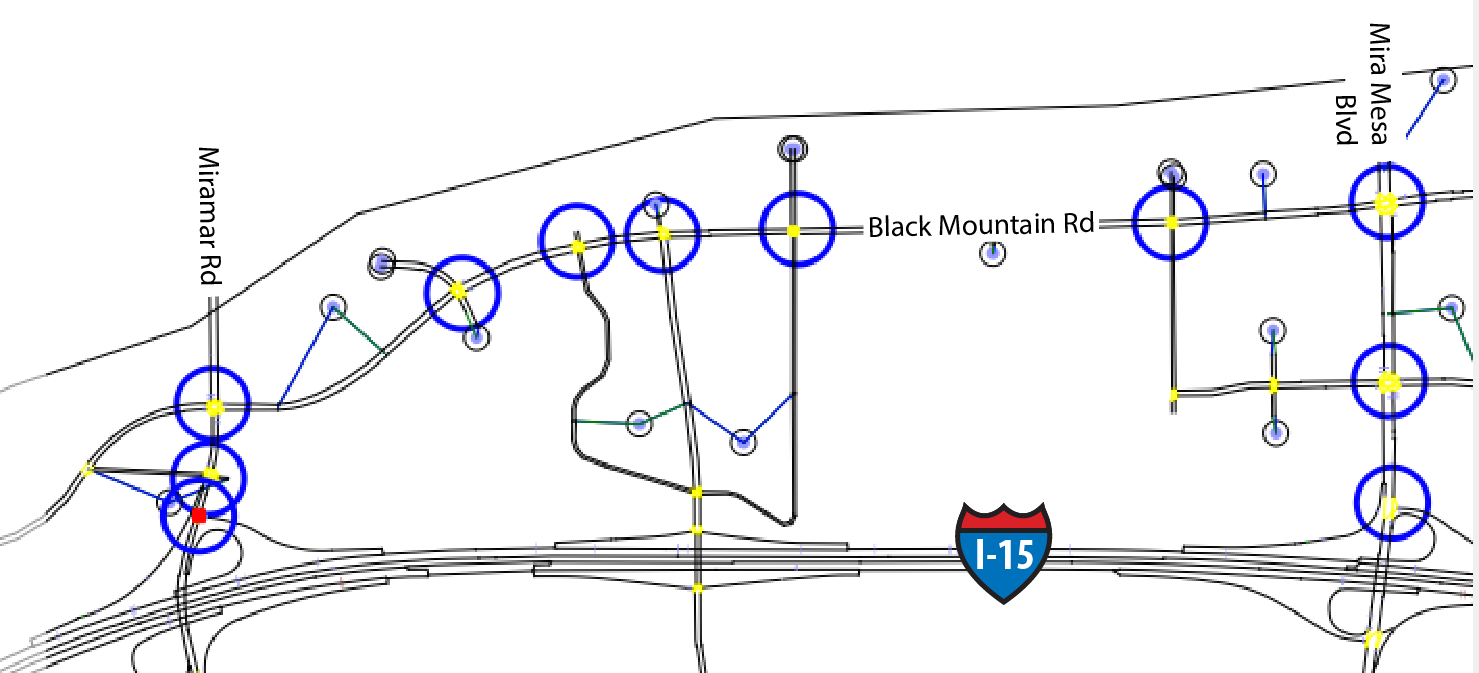
\includegraphics[width=.8\columnwidth]{./i15network.png}
\caption{The chosen network was calibrated to represent realistic demands and physical parameters observed on a stretch of Black Mountain Road near the I-15 freeway in San Diego, California.}
\vspace{-1em}
\end{figure}
%
%The remainder of this section provides a comparison of the performance of the cycle-based max pressure algorithm with two other control algorithms described below. While it makes sense to compare the numerical performance of these algorithms, it should be noted that while the other algorithms seem to perform well in simulation, they come with no proof or theoretical guarantees on operation.
Various performance metrics were compared between model runs using the max pressure controller and two alternative controllers: a fixed-time control plan that divides each signal cycle equally between all available phases, and a ``fully-actuated'' control system such as that which is currently operational on the real road network represented by the model. The fully actuated-controller is essentially a flexible fixed-time plan in which green times can be shortened or extended in real time to promote continuity of flows in response to instantaneous link demand measurements. 
%\begin{figure}[h!]
%\centering
%\includegraphics[width=\columnwidth]{./AIMSUN_intersection.png}
%\caption{Cycle-allocated max pressure was implemented using a cycle length of 90 seconds and minimum time constraints of 10 seconds for each phase.}
%\end{figure}
The comparison of network vehicle counts in Figure \ref{fig_counts} suggests that the uniformly-allocated fixed time controller caused significantly fewer vehicles to be served than the other two controllers, which were comparable to each other in vehicle service rates. This difference made it difficult to fairly compare other performance metrics between the uniform fixed-time controller and the other two options. 
\begin{figure}[h!]
\centering
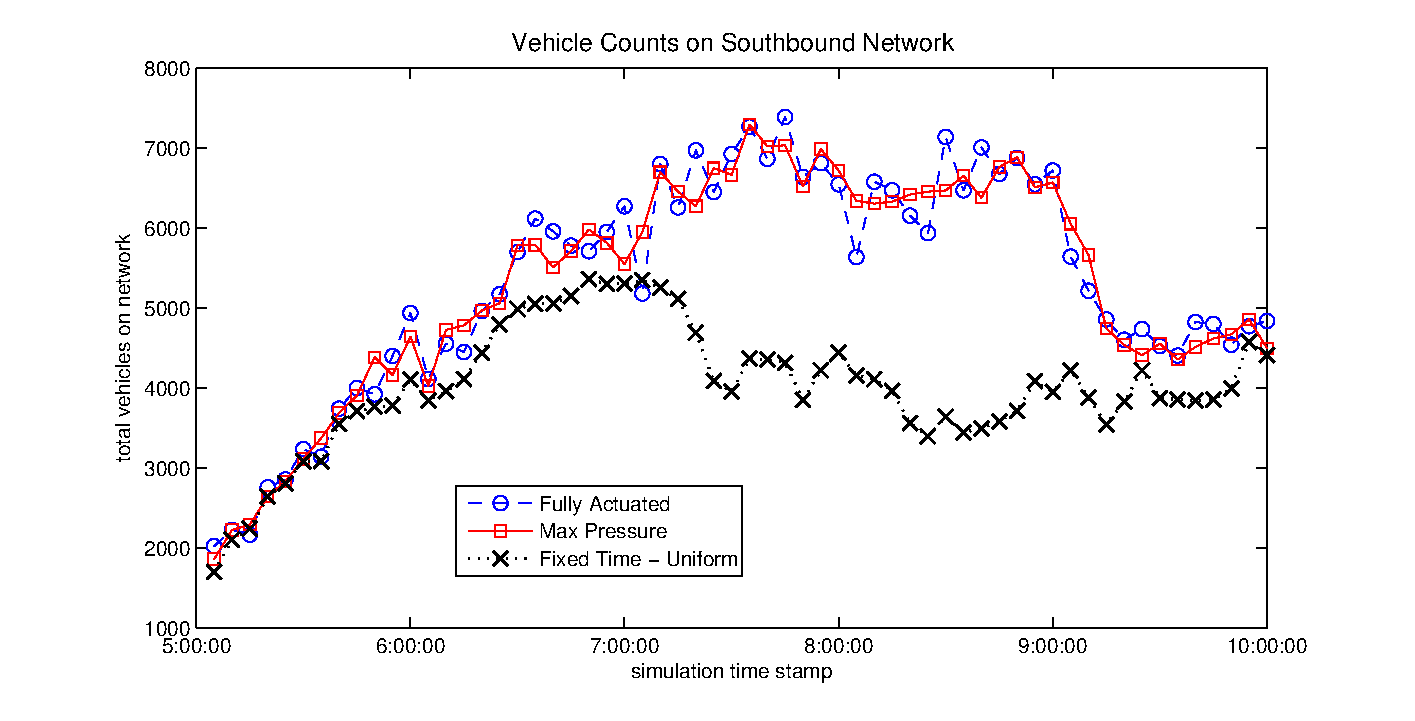
\includegraphics[width=\columnwidth]{./VehicleCountsPlot.eps}
\vspace{-2em}
\caption{During congestion, cycle-based max pressure demonstrated service rates that are higher than the uniformly allocated fixed-time controller and consistent with a fully-actuated control system.  \label{fig_counts}}
\end{figure}
\begin{figure}[h!]
\vspace{-2em}
\centering
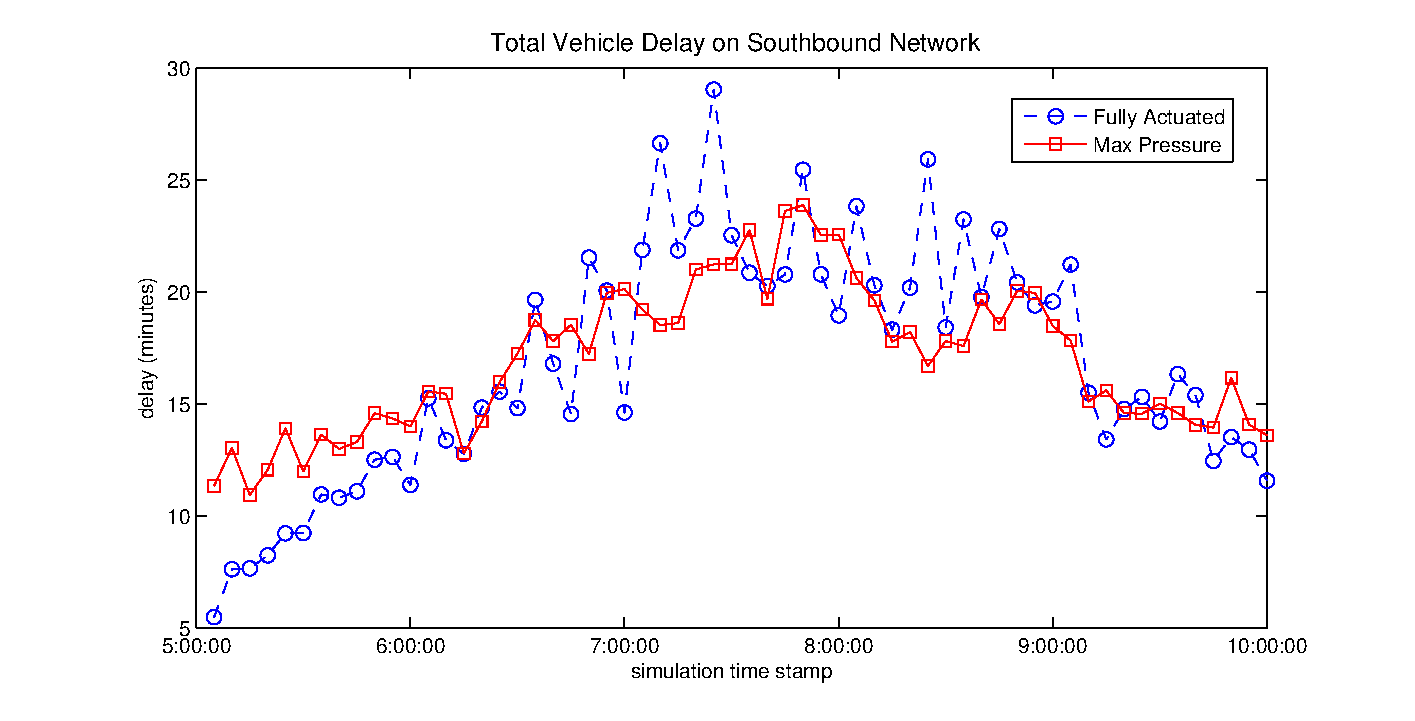
\includegraphics[width=\columnwidth]{./VehicleDelayPlot.eps}\\
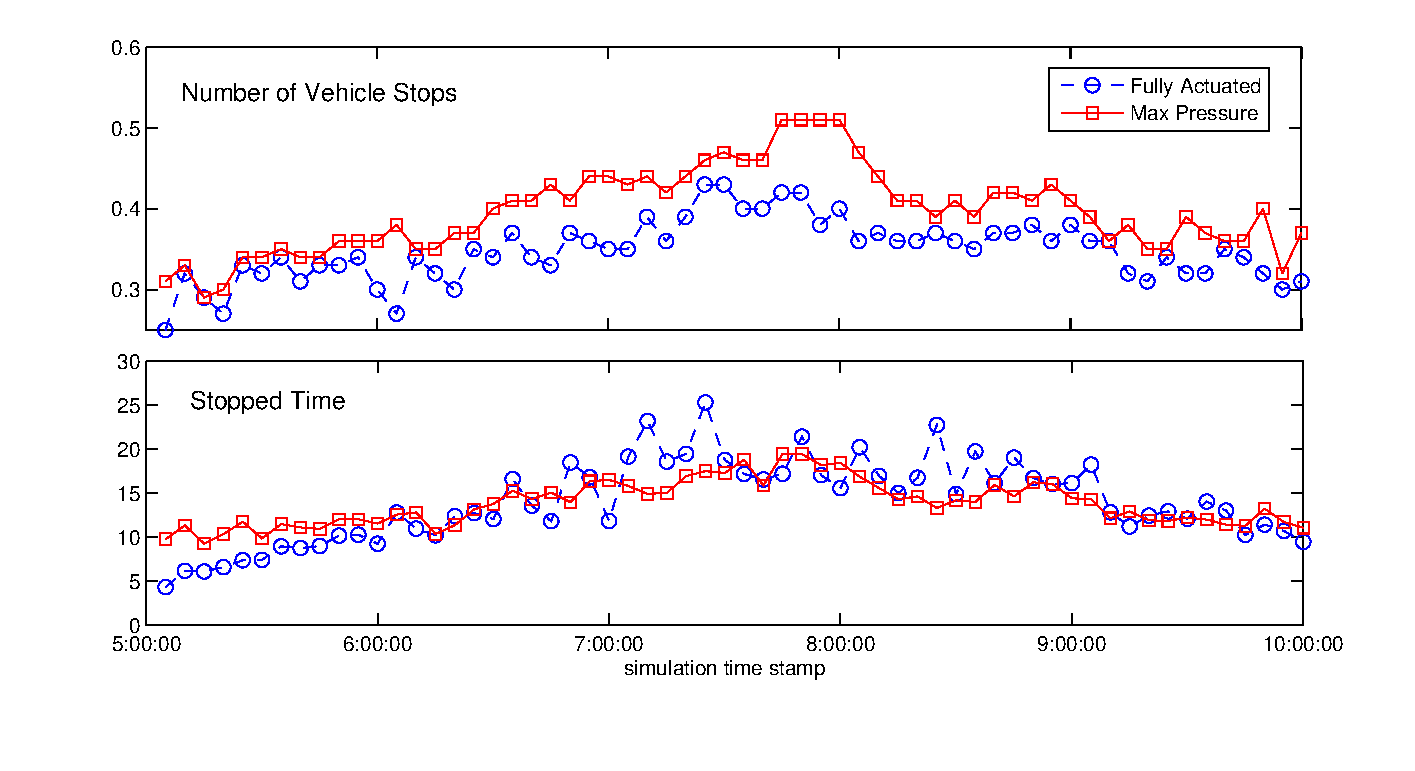
\includegraphics[width=\columnwidth]{./VehicleStopsPlot.eps}
\vspace{-2.5em}
\caption{Cycle-based max pressure outperforms the fully actuated system during periods of high demand. While max pressure caused more vehicle stop events, stoppage times were similar to those observed using the standard fully-actuated controller. \label{fig_delaystops}}
\end{figure}

Differences between the fully-actuated and cycle-based max pressure controllers were observed in measurements of delays and queue lengths: while the fully-actuated system appeared to produce less delay and shorter queues than max pressure during periods of relatively low network demand, max pressure was equally as effective or even more effective at reducing delays and queue lengths given larger demands. Figure \ref{fig_delaystops} shows how delays were reduced and had less variance over time when the max pressure controller was applied than with the fully-actuated controller. 
However, cycle-based max pressure consistently induced more stops during a vehicle's journey across the network, which is expected given the design objectives of the fully-actuated system. Total stoppage times were higher with max pressure given low demand, but improved over the existing controller during peak demand. 
%\begin{figure}[h!]
%\centering
%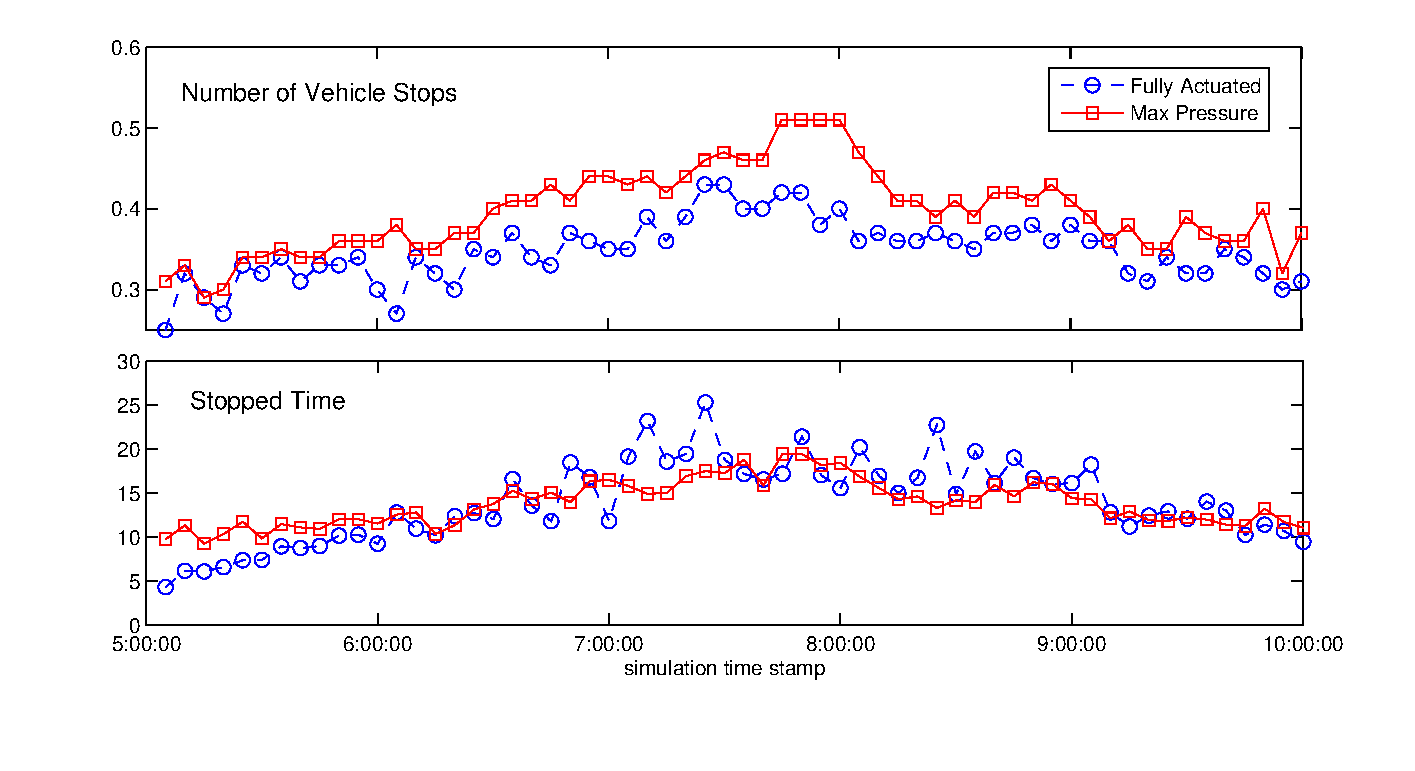
\includegraphics[width=\columnwidth]{./VehicleStopsPlot.eps}
%\vspace{-2.5em}
%\caption{While max pressure caused more vehicle stop events, stoppage times were similar to those observed using the standard fully-actuated controller.\label{fig_stops}}
%\end{figure}





\section{Conclusion}
In this work we have defined an extension of the max pressure controller required for application on a real network of signalized traffic intersections. Given only the constraint that the network demands are serviceable in average, we have proven that updating a max pressure controller which allocates a fixed minimum proportion of service to each permissible phase at a slower rate than that which governs traffic flow will not destroy the stabilizing properties of the controller. 

%While there are additional modifications to the control model that must be addressed before max pressure can be considered a feasible algorithm for real-time operation of traffic signal controllers, 
Max pressure provides theoretical guarantees on network-wide performance that are lacking in other existing signal control algorithms. Our implementation in the referenced micro-simulation platform furthermore demonstrates how it could comply with the hardware and communications constraints commonly encountered in existing roadway infrastructure. These numerical simulations  reveal that an implementation of cycle-based max pressure competes with the existing standard feedback controller in many performance metrics, especially during periods of high congestion. It also appears to provide less variance in delays than the existing alternative. Future work will involve further analysis of the effect of cycle length on the performance of cycle-based max pressure, as well as performance improvements that can be achieved via the addition of common signal coordination practices in a network running cycle-based max pressure. 
% if have a single appendix:
%\appendix[Proof of the Zonklar Equations]
% or
%\appendix  % for no appendix heading
% do not use \section anymore after \appendix, only \section*
% is possibly needed
% use appendices with more than one appendix
% then use \section to start each appendix
% you must declare a \section before using any
% \subsection or using \label (\appendices by itself
% starts a section numbered zero.)
%
% you can choose not to have a title for an appendix
% if you want by leaving the argument blank
% use section* for acknowledgement
\vspace{-.5em}
\section*{Acknowledgments}
This work was sponsored by the California Department of Transportation under the Connected Corridors program at UC Berkeley PATH. The authors would like to thank Pravin Varaiya for his insights on this work, as well as Brian Peterson and Joe Butler for their support in the implementation.
% Can use something like this to put references on a page
% by themselves when using endfloat and the captionsoff option.
\ifCLASSOPTIONcaptionsoff
  \newpage
\fi
% trigger a \newpage just before the given reference
% number - used to balance the columns on the last page
% adjust value as needed - may need to be readjusted if
% the document is modified later
%\IEEEtriggeratref{8}
% The "triggered" command can be changed if desired:
%\IEEEtriggercmd{\enlargethispage{-5in}}

% references section

% can use a bibliography generated by BibTeX as a .bbl file
% BibTeX documentation can be easily obtained at:
% http://www.ctan.org/tex-archive/biblio/bibtex/contrib/doc/
% The IEEEtran BibTeX style support page is at:
% http://www.michaelshell.org/tex/ieeetran/bibtex/
%\bibliographystyle{IEEEtran}
% argument is your BibTeX string definitions and bibliography database(s)
%\bibliography{IEEEabrv,../bib/paper}
%
% <OR> manually copy in the resultant .bbl file
% set second argument of \begin to the number of references
% (used to reserve space for the reference number labels box)
%\begin{thebibliography}{1}
%
%\bibitem{varaiyaStochastic}
%P.~Varaiya, \emph{Max pressure control of a network of signalized intersections}, FINISH THIS BIB ITEM
%
%\end{thebibliography}

\bibliographystyle{IEEEtran}
\bibliography{mp_references}

% biography section
% 
% If you have an EPS/PDF photo (graphicx package needed) extra braces are
% needed around the contents of the optional argument to biography to prevent
% the LaTeX parser from getting confused when it sees the complicated
% \includegraphics command within an optional argument. (You could create
% your own custom macro containing the \includegraphics command to make things
% simpler here.)
%\begin{biography}[{\includegraphics[width=1in,height=1.25in,clip,keepaspectratio]{mshell}}]{Michael Shell}
% or if you just want to reserve a space for a photo:

\appendices
\section{Feasible flows with a $\tau$-updated controller}
% !TEX root = ./MParticle_resubmit.tex
\label{tauadmissible}
%We first prove that this set of $\tau$-admissible flows (demands that can be accommodated using $\tau$-non updated sequences) is in fact the same set of flows that is admissible under typical updated control sequences, defined in equation \eqref{feasible_demand}. 
\begin{Lem}
All flows which satisfy Property \ref{feasible_property} given a controller $u$ updated at every model time step will also satisfy Property \ref{feasible_property} with a $\tau$-updated controller for some $\tau$. 
\end{Lem}
\begin{proof}
Given the set admissible phases $U$, define:
\begin{itemize}
\item $\mathcal U$ is the set of control sequences with distinct elements $\{S(1), S(2) \ldots S(t) \ldots |  S(\cdot) \in U\} $,
\item $\mathcal U_{\tau}$ is the set of $\tau$-updated control sequences $\{S(1), S(1), \ldots ,  S(\tau + 1),S(\tau + 1), \ldots , S(n\tau + 1), \\  S(n\tau + 1), \ldots |  S(\cdot) \in U\} $, 
\end{itemize}
Also define the following sets of \emph{long-term control proportion matrices}, which are similar to the formulation in \eqref{longterm_proportion}:
\vspace{-.5em}
\begin{small}
\begin{align*} M_{\mathcal U} = \Big\{\lim \inf_{T}\dfrac{1}{T}\sum_{t=1}^{T}  S&(t)  \Big| \{S(1), S(2), \ldots, S(t), \ldots \}\in \mathcal U \Big\} \end{align*}
\vspace{-1em}
\begin{align*} M_{\mathcal U_\tau} = \Big\{\lim&\inf_{T} \dfrac{1}{T}\sum_{t=1}^{T} S(t) \; \cdot \\ 
& \Big|\{S(1), S(1), \ldots,  S(\tau+1),S(\tau+1), \ldots\}\in \mathcal U_{\tau} \Big\} \end{align*}
\end{small}
By Property \ref{feasible_property}, a demand $d$ is only feasible if there exists a control sequence $\overline {S}$ such that the corresponding long-term control proportion matrix $M_{\overline {S}}$ satisfies \eqref{feasible_demand}. Here we show $M_{\mathcal U} = M_{\mathcal{U_\tau}}$, and therefore any flows that are admissible given an unrestricted controller in $\mathcal U$ can also be accommodated using a $\tau$-updated controller in $\mathcal{U}_\tau$. 

Obviously, $M_{\mathcal U_\tau}  \subset M_{\mathcal U}$. To show equality, we must also demonstrate that $M_{\mathcal U}  \subset M_{\mathcal {U}_\tau} $. Suppose there exists a control sequence $\hat{S} = \{ S(1), S(2), \ldots \} \in \mathcal{U}$. 
By definition, \begin{small}
\begin{align*}
M_{\hat{S}} &= \lim\inf_{T} \dfrac{1}{T}\sum_{t=1}^{T} S(t) = \lim\inf_{T} \dfrac{1}{\tau T}\sum_{t=1}^{\tau T}  \tilde{S}(t) \; \\ 
& \qquad \text{ where } \tilde{S} = \{S(1), S(1), \ldots, S(t), S(t), \ldots \} \\
&= \lim\inf_{T} \dfrac{1}{ T}\sum_{t=1}^{T}  \tilde{S}(t) \in M_{U_\tau}  \quad \implies M_{\mathcal U}  \subset M_{\mathcal {U}_\tau}
\end{align*}\end{small}
\end{proof}
 

%\begin{IEEEbiography}{Thomas Pumir}
%received a BSc in mathematics from
%Ecole Normale Sup\'erieure, Cachan, France in July
%2011, the M.S. in Probability and Statistics from Universit\'e Paris Sud, Orsay, France in September 2012
%and the M.S. in applied mathematics from Ecole
%Normale Sup\'erieure, Cachan, France in September
%2013. He is currently working towards the PhD
%degree at the department of Operations Research and
%Financial Engineering at Princeton University, NJ.
%\end{IEEEbiography}
%
%\begin{IEEEbiography}{Leah Anderson}
%is a PhD student in systems engineering
%at the University of California, Berkeley. She
%received a B.S. in engineering from Harvey Mudd
%College in 2009, and a M.S. in civil systems engineering
%from UC Berkeley in 2010. Her research
%interests include real-time estimation and control
%in distributed sensing applications. She specifically
%works with related problems in water flow and road
%traffic networks.
%\end{IEEEbiography}
%
%% insert where needed to balance the two columns on the last page with
%% biographies
%%\newpage
%
%\begin{IEEEbiography}{Alexandre M. Bayen} 
%received the Engineering degree in applied mathematics from the Ecole Poly- technique, Palaiseau, France, in July 1998, the M.S. and Ph.D. degrees in aeronautics and astronautics from Stanford University, Stanford, CA, USA, in June 1999 and December 2003, respectively.
%He was a Visiting Researcher at NASA Ames Research Center from 2000 to 2003. He worked as the Research Director of the Autonomous Naviga- tion Laboratory at the Laboratoire de Recherches Balistiques et Aerodynamiques, (Ministere de la
%Defense, Vernon, France), where he holds the rank of Major. He is an Associate Professor of Electrical Engineering and Computer Sciences at the University of California Berkeley, Berkeley, CA, USA. He has authored one book and over 100 articles in peer reviewed journals and conferences.
%Dr. Bayen is the recipient of the Ballhaus Award from Stanford University in
%2004, of the CAREER Award from the National Science Foundation in 2009,
%and is a NASA Top 10 Innovators on Water Sustainability, 2010. His projects
%Mobile Century and Mobile Millennium received the 2008 Best of ITS Award
%for Best Innovative Practice, at the ITS World Congress and a TRANNY Award
%from the California Transportation Foundation, 2009. He is the recipient of the
%Presidential Early Career Award for Scientists and Engineers (PECASE) Award
%from the White House in 2010. Mobile Millennium has been featured more
%than 100 times in the media, including TV channels and radio stations (CBS,
%NBC, ABC, CNET, NPR, KGO, the BBC), and in the popular press (Wall Street
%Journal, Washington Post, LA Times).
%\end{IEEEbiography}

% You can push biographies down or up by placing
% a \vfill before or after them. The appropriate
% use of \vfill depends on what kind of text is
% on the last page and whether or not the columns
% are being equalized.

%\vfill

% Can be used to pull up biographies so that the bottom of the last one
% is flush with the other column.
%\enlargethispage{-5in}


\end{document}


